%------------------------------------------------
\chapter{\textbf{Projeto \textit{hardware} e \textit{software} do Micromouse}}\label{ProjetoDosModulos}
%---------------------------------------------------------

\section{Introdução}
O projeto de uma solução para atender todo o requisito de uma competição Micromouse exige atenção tanto no projeto \textit{hardware} como no \textit{software}: ambos em sintonia perfeita. Para tanto, no quesito \emph{hardware}, é necessário que o cerebro microcontrolador do Micromouse tenha boa velocidade na execução do algoritmo, boa RAM (ao menos 4 KB de RAM), com módulos específicos QEI para decodificação de pulsos por quadratura dos \emph{encoders} por \textit{hardware}, e baixo consumo de energia. Já no quesito \emph{software}, o algoritmo deve ser otimizado para o consumo mínimo de RAM, uma vez que o mesmo depende bastante de estruturas de dados e pilhas para executá-lo.

Na Figura \ref{fig:system_completo} é apresentado o diagrama do projeto proposto. Pode-se perceber que todos os processos são controlados pelo microcontrolador, o cerebro do robô. No diagrama, são observados módulos de \emph{hardware} e de \emph{software} essenciais. 

\begin{figure}[!htb]
	\caption{\label{fig:system_completo}Diagrama de blocos do sistema robótico Micromouse}
	\begin{center}
		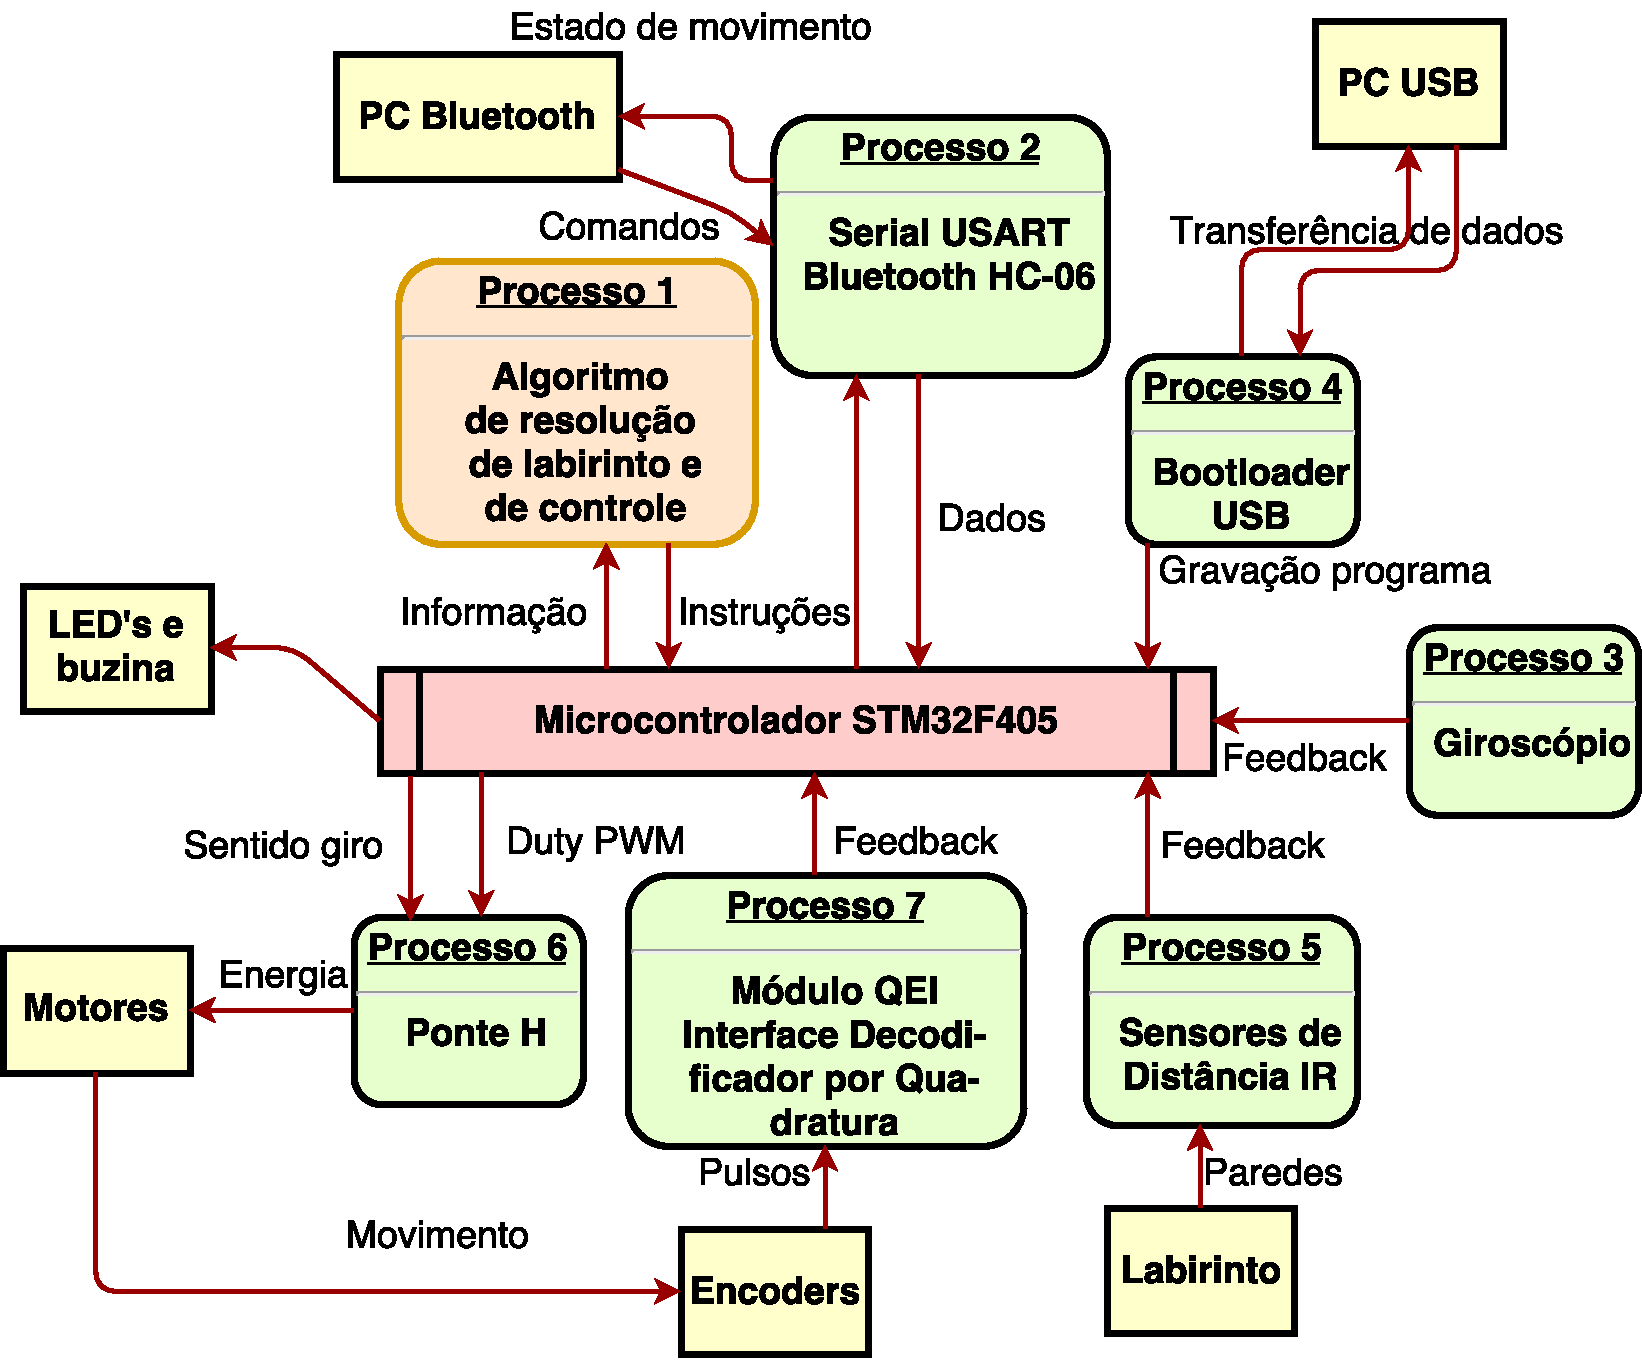
\includegraphics[width=0.7\linewidth]{diagrama_geral.pdf}
	\end{center}
	\legend{Fonte: autor (2017)}
\end{figure}

Todos os processos mostrados na figura, (exceto o processo 1), fazem parte do microcontrolador do robô e do chassi do mesmo, sendo estes módulos projetos de \textit{hardware}. A implementação das partes de algoritmo para resolução de labirinto e para controle de trajetórias está representada como instruções de programa (processo 1). A requisição de dados de \emph{feedback} dos \emph{ecoders} (processo 7), do giroscópio e das paredes (processos 3 e 5), envio de dados por \textit{bluetooth} (processo 2), e controle dos Motores (processo 6) são controlados pelo processo 1. As setas mostram os fluxos de dados entre os módulos e o microcontrolador.

O projeto foi dividido em três partes: \textit{hardware}, algoritmo e controle. Em todos os robôs de \citeonline{5971240}, \citeonline{remendo3}, \citeonline{remendo1}, \citeonline{6852576}, \citeonline{lin2010design}, \citeonline{7344099} utilizaram-se destas partes. No entanto, embora a parte de \emph{hardware} esteja como parte do projeto proposto, somente são citados os componentes do robô adquirido, e não foi construído por este trabalho.

Existem diversos projetos \emph{open source} prontos para uso para competições deste tipo e para competições para seguidores de linha. Hoje, os fãs da competição não precisam mais construir os seus robôs a partir do zero. Peças, kits e projetos \emph{open source} completos estão disponíveis no mercado \cite{Christian:2014}. Por exemplo, a Figura \ref{fig:opensource_micro} mostra o chassi Micromouse para uso com placas Arduíno e é comum de se achar no mercado. Para este trabalho, foi adquirido o projeto \emph{uMaRT Lite Plus} de Figura \ref{fig:robo1}. 


\begin{figure}[!htb]
	\caption[Micromouses open source prontos para uso]{\label{fig:opensource_micro}Micromouses didáticos disponíveis no mercado}
	\begin{center}
		\subfloat[Micromouse com Arduino]{\includegraphics[width=0.4\linewidth]{arduino_Micromouse.jpg}}
		\hspace*{0.1\linewidth}
		\subfloat[Micromouse Ioton Brasil]{\includegraphics[width=0.4\linewidth]{Micromouse-ioton.png}}
	\end{center}
	\legend{Fonte: autor (2017)}
\end{figure}

Quanto ao algoritmo de resolução de labirintos (Segunda parte), na literatura, é comum o uso do algoritmo de imundação \emph{Flood Fill}. Dentre os três algoritmos mais estudados (Seguidores de parede, Tréumax e \emph{Flood Fill}), o algoritmo preferido por todos consegue resolver perfeitamente qualquer que seja o \emph{design} do labirinto, enquanto que os algoritmos mais simples não o fazem, conforme pode se observar nas Figuras \ref{fig:traj_seguidor} e \ref{fig:traj_flood} a comparação entre ambos os algoritmos para labirinto que não tem paredes ligadas entre si até o centro (as células em cinza não foram visitadas - o seguidor de parede não resolve o labirinto). Portanto, a justificativa para o desenvolvimento, simulação e implementação do algoritmo \emph{Flood Fill} para este projeto é a eficiência na resolução de qualquer configuração de labirinto em uma eventual competição.

\begin{figure}[!htb]
	\caption{\label{fig:traj_seguidor}Trajetória do algoritmo Seguidor de parede}
	\begin{center}
		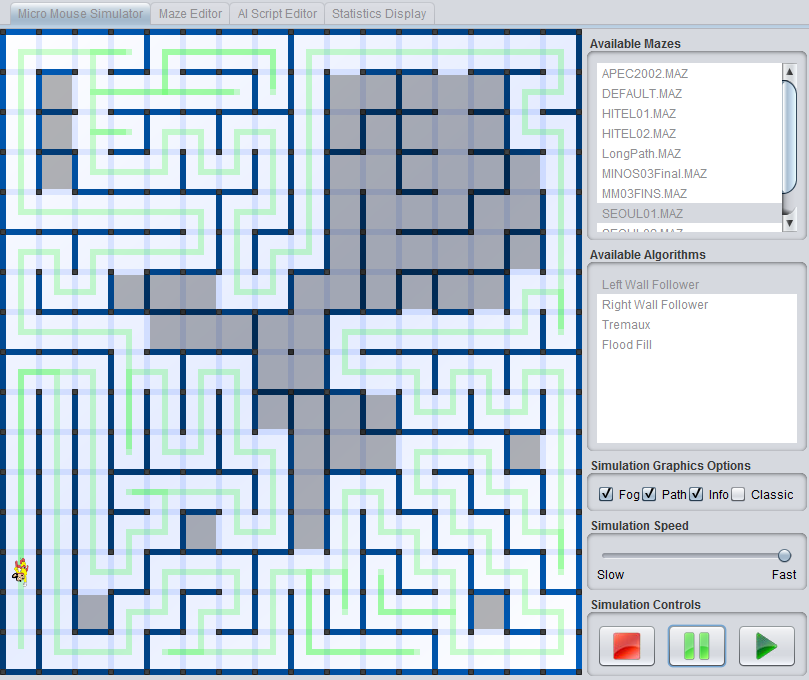
\includegraphics[width=0.8\linewidth]{seguidor_parede.png}
	\end{center}
	\legend{Fonte: autor (2017)}
\end{figure}


Já a terceira parte é o projeto de controlador de velocidades das rodas, em malha fechada. Como o sistema não é ideal, o robô pode sofrer interferências externas, como ruído, deslizamento das rodas, entre outros, de forma que a trajetória projetada para os perfis de reta e curva se altere em \emph{malha aberta}, ou seja, o robô poderá sair da trajetória e perder sua referência no labirinto. Uma das formas para correção deste problema, outro controle realimentado foi construído, sendo que a sua realimentação é a informação do giroscópio e/ou dos sensores de distância. A construção de perfis de curvas, e integração dos sensores de distância e \emph{encoders}, é de fundamental importância, a fim de atuar corretamente os motores de forma que siga a trajetória pré determinada pelo algoritmo.

Portanto, o sucesso em uma eventual competição desta modalidade depende da construção das partes citadas.

\begin{figure}[!htb]
	\caption{\label{fig:traj_flood}Trajetória do algoritmo \emph{Flood Fill}}
	\begin{center}
		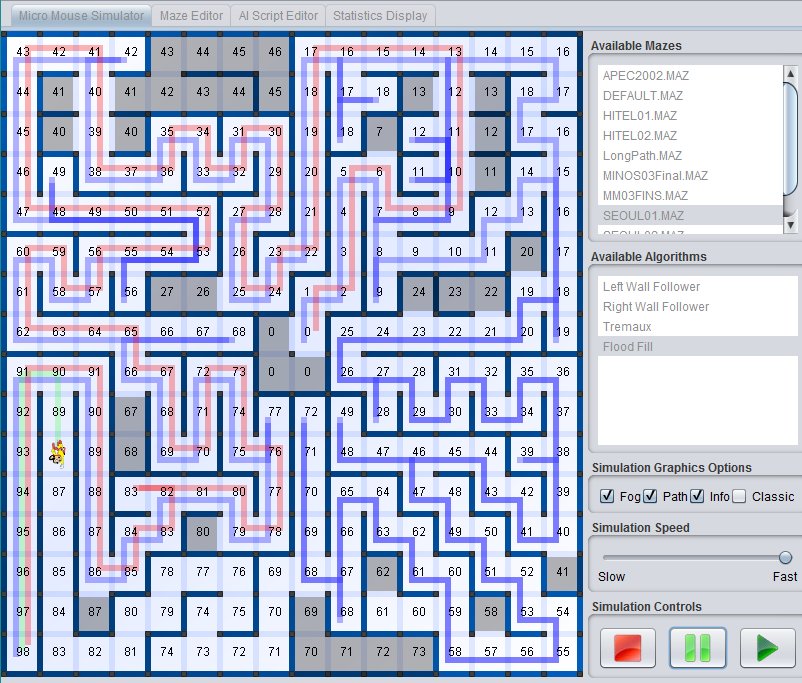
\includegraphics[width=0.8\linewidth]{caminho_flood_fill.png}
	\end{center}
	\legend{Fonte: autor (2017)}
\end{figure}


\section{Hardware - o robô Micromouse}
O robô tem como objetivo encontrar o centro do labirinto, onde estão as quatro células-alvo. Após esta corrida, o robô deve mapear o melhor caminho para melhorar seu tempo de corrida no sentido de alcançar o menor tempo possível, sendo que o ganhador é o robô que fez o menor tempo de corida da célula de partida até as células-alvo.


\subsection{Componentes do robô}
A perspectiva de todo o sistema pode ser visto pela Figura \ref{fig:arranjo}, onde mostra todos os componentes necessários para o robô operar de forma satisfatória num labirinto. O robô tem um microcontrolador conectado com os periféricos sensoriais e motores. O cerebro do robo, o microcontrolador, será capaz de verificar obstáculos à frente com os sensores de distância, tomar decisões e atuar ajustando as velocidades dos motores. A autonomia é garantida pela bateria. Então, o robô recebe informações dos sensores e processa-os de forma a comandar corretamente os motores.


A plataforma robótica utilizada é ideal para desenvolvimento de projetos de solucionadores de labirinto. O robô denominado \emph{uMaRT Lite Plus}, de Figura \ref{fig:robo1}, é um kit educacional de robótica destinado ao aprendizado e utiliza o microcontrolador da ARM STM32F405.

\begin{figure}[!htb]
	\caption{\label{fig:robo1}Vista superior do robô \emph{uMaRT Lite Plus}}
	\begin{center}
		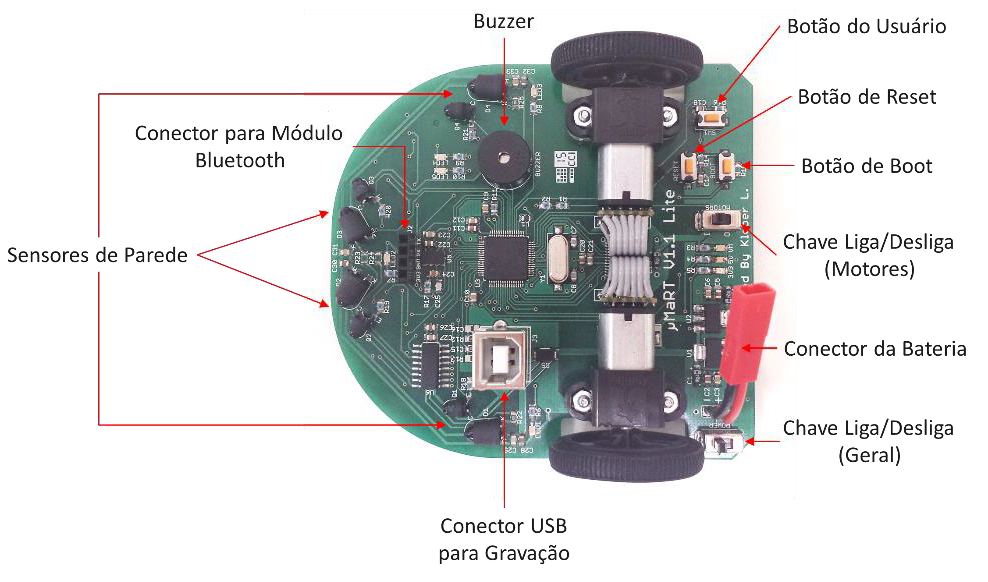
\includegraphics[width=0.8\linewidth]{robo1.png}
	\end{center}
	\centering
	\small Fonte: adaptado de \citeonline{umart:2015}
\end{figure}


As informações técnicas são as seguintes:

\begin{enumerate}[leftmargin=2cm,label=\alph*)]
	\item dimensões (comprimento, largura, altura): 95x89x32 $~mm$;
	\item peso (sem bateria): 71$~g$;
	\item bateria: Li-Po 300 $~mAh$ de duas células;
	\item microcontrolador: STM32F405RGT6, com $192~kB$ de RAM e $168~MHz$;
	\item tensão de entrada (bateria): 6 - 9 $~V$;
	\item motores: micromotor Pololu com caixa de redução de metal 30:1 HP (1000 RPM);
	\item rodas: 32x7mm (plástico e borracha);
	\item \textit{encoders}: magnético em quadratura (360 PPR);
	\item sensores de linha: QRE1113GR;
	\item sensores de parede: SRH4545 (LED)/TEFT4300 (fototransistor);
	\item giroscópio: LY3200ALH;
	\item ponte H dos motores: TB6612FNG.
\end{enumerate}

Esta plataforma robótica é completa e de alto desempenho. Ela conta com dois micromotores com caixa de redução de metal, \textit{encoders} independentes de 360 pulsos por revolução (PPR), oito sensores de linha, quatro sensores de parede, buzzer, medição da tensão da bateria, giroscópio, conector para depuração ou controle sem fio via módulo \textit{bluetooth}, um botão e cinco LEDs para interação com o usuário. Capaz de atingir velocidades de até 2,0m/s, o uMaRT Lite Plus é um ótimo kit para o aprendizado e para utiliza-lo em competições de robótica.

Este robô contém dois módulos QEI (\textit{Quadrature Encoder Interface}), incomum em microcontroladores baratos. Este módulo permite, quando ligado a um \textit{encoder} mecânico ou óptico, dar informação acerca da direção da rotação e do número de pulsos realizados. Os \textit{encoders} magnéticos emitem dois sinais: Fase A e Fase B. Se a fase A está em avanço em relação à fase B, o sentido de rotação é positivo e, em caso contrário, o sentido de rotação é considerado negativo.

\subsection{Programação}
Umas das maneiras de programar microcontroladores da plataforma ARM é por meio do \textit{software} \textit{ECLIPSE IDE}. No \textit{site} Micromouse Brasil (em Arquivos) são disponibilizados tutoriais de configuração e criação de projeto. Também serão fornecidos alguns exemplos básicos de código em repositórios no GitHub: github.com/Micromousebrasil. Os códigos de programação são construídos em linguagem C.

No projeto teste fornecido pelo fabricante do robô, constam algumas funções básicas implementadas, prontas para uso, funções estas que retornam valores importantes para uso em algoritmos de controle como realimentadores do processo em malha fechada e para detecções de obstáculos durante uma corrida em labirinto. As seguintes funções foram utilizadas em conjunto com os algoritmos de controle e de resolução de labirinto.

\begin{enumerate}[leftmargin=2cm,label=\alph*)]
	\item \verb+getSensoresParede()+: função que retorna, em binário, se existem paredes à frente do robô. São três \emph{bits} de informações, sendo que o \emph{bit} mais significativo representa a existência da parede à esquerda, o segundo \emph{bit}, parede à frente, e, por último, o \emph{bit} menos significativo identifica a existência da parede à direita;
	\item \verb+getSensoresLinha()+: utilizado para ler informações dos sensores leitores de linha. Função não utilizada e retirada do programa;
	\item \verb+getGyro()+: utilizado para retornar o valor de grandeza proporcional ao valor de velocidade angular global do robô;
	\item \verb+getTensao()+: função que retorna o valor de tensão da bateria. Utilizado para detectar o momento certo de carregar a bateria;
	\item \verb+setMotores(int16_t pwm_esquerda, int16_t pwm_direita)+: função utilizada pelo controlador para atualizar o sinal de controle das rodas;
	\item \verb+setLED(Led_TypeDef led, GPIO_PinState estado)+: utilizado para acender ou apagar algum LED do Micromouse. No robô existem 5 LEDs;
	\item \verb+toggleLED(Led_TypeDef led)+: utilizado para alternar o estado do LED;
	\item \verb+allLEDs(GPIO_PinState estado)+: utilizado para acender ou apagar todos os {LEDs} do Micromouse. Geralmente utilizado no final de uma corrida. É uma forma de alerta de êxito;
	\item \verb+getEncoderEsquerda(void)+: utilizado para obter a quantidade de pulsos gerados pelo \emph{encoder} conectado ao eixo do motor esquerdo. Útil para realimentar o controle de velocidade das rodas;
	\item \verb+resetEncoderEsquerda(void)+: utilizado para zerar a quantidade de pulsos armazenados pelo contador do módulo QEI;
	\item \verb+getEncoderDireita(void)+: utilizado para obter a quantidade de pulsos gerados pelo \emph{encoder} conectado ao eixo do motor direito. Útil para realimentar o controle de velocidade das rodas;
	\item \verb+resetEncoderDireita(void)+: utilizado para zerar a quantidade de pulsos armazenados pelo contador do módulo QEI.
\end{enumerate}

\subsection{Gravação}
O ARM STM32F405 do robô uMaRT Lite Plus pode ser gravado por Bootloader em dois modos, USART 1 (conector J2) ou USB-DFU (conector J3). Para que o microcontrolador entre no modo de boot é necessário resetar o microcontrolador com o botão de BOOT pressionado, logo após este procedimento o botão de BOOT já pode ser liberado e o microcontrolador já está no modo de gravação via Bootloader. 
\begin{enumerate}[leftmargin=2cm,label=\alph*)]
\item \textit{software} de gravação via USART: STMFlashLoader;
\item \textit{software} de gravação via USB: DfuSe USB.
\end{enumerate}

\subsection{Comunicação}
O STM32F405 possui conectividade USB 2.0 \textit{full-speed} e \textit{high-speed} que pode ser usada para comunicação com um computador.
Outro tipo de comunicação com um computador ou com um smartphone é por meio de um módulo \textit{bluetooth} HC-06 conectado ao conector J2.

\subsection{Cinemática do robô móvel diferencial}
O robô Micromouse, Figura \ref{fig:robo1}, é um robô móvel com tração diferencial, isto é, as rodas são acionadas independentemente. A tração diferencial tem as seguintes características:
\begin{enumerate}[leftmargin=2cm,label=\alph*)]
	\item rodas co-axiais;
	\item tracionadas independentemente;
	\item duas dimensões;
	\item restrito holonomicamente.
\end{enumerate}

\begin{figure}[!hb]
	\caption{\label{fig:robo_dif_carac}Robô móvel diferencial - características}
	\begin{center}
		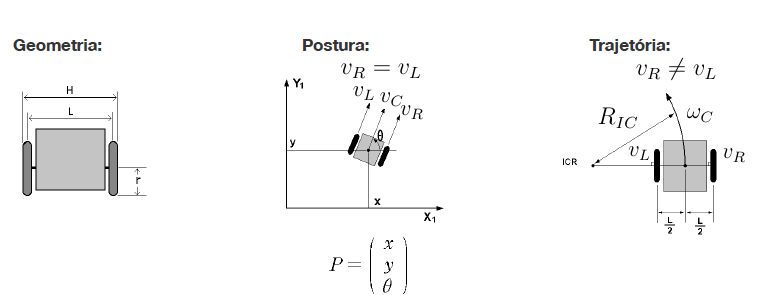
\includegraphics[width=0.9\linewidth]{robo_diferencial_carac.png}
	\end{center}
	\centering
	\small Fonte: autor (2017)
\end{figure}

Como pode-se perceber na Figura \ref{fig:robo_dif_carac}, o robô diferencial depende de sua geometria (distância entre as rodas e o raio das mesmas) para o cálculo de postura ($x$, $y$ e $\theta$) e de previsão de trajetória.
	
Quando as duas rodas tem suas velocidades iguais, o robô realiza uma linha reta ($v_R = v_L$, onde $v_R$ e $v_L$ são, respectivamente, as velocidades da roda direita e da roda esquerda). Quando as velocidades são diferentes ($v_R \neq v_L$), a sua trajetória forma um arco. E para realizar um giro em torno do seu eixo, as velocidades são iguais, mas com os sentidos trocados ($v_R = -v_L$). A restrição holonômica é quando sua posição é limitada a um subconjunto do espaço de configurações através de uma função igual a zero.

A cinemática direta de um robô móvel diferencial é caracterizada através das Equações (\ref{eq:veloc_v}) e (\ref{eq:veloc_w}). Dada a geometria do robô e a velocidade das rodas, determinam-se as velocidades linear e angular global, além do ângulo de direção num plano bidirecional, conforme é mostrado na Figura \ref{fig:robo_dif_cinematica}, onde $r$ é o raio das rodas, $L$ é a largura do eixo, $v_R$ é a velocidade angular da roda direita e $v_L$ é a velocidade angular da roda esquerda. 


\begin{figure}[!hb]
	\caption{\label{fig:robo_dif_cinematica}Robô móvel diferencial - cinemática direta}
	\begin{center}
		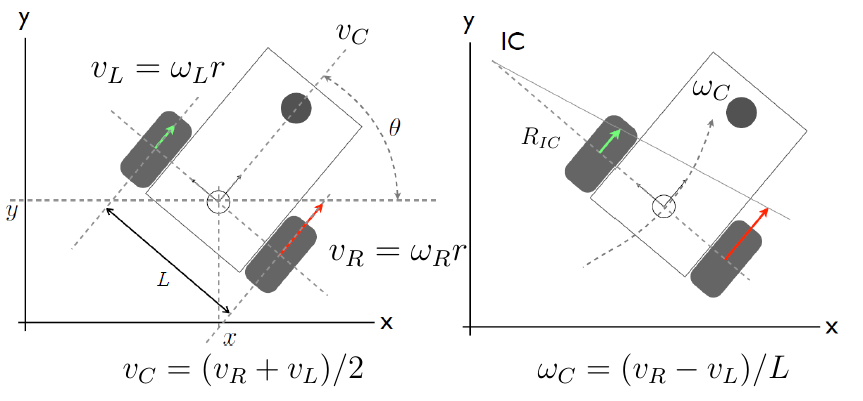
\includegraphics[width=0.8\linewidth]{robo_diferencial_cinematica.png}
	\end{center}
	\centering
	\small Fonte: autor (2017)
\end{figure}

Seguindo pelas equações cinemáticas, pode-se calcular a velocidade angular para velocidade linear e raio de curvatura fixas ($\omega_C = v_C/{R_{IC}}$), onde $R_{IC}$ é o raio do centro instantâneo da trajetória circular. O controlador proposto ajusta as velocidades das rodas de tal maneira a fixar as velocidades calculadas e o robô seguirá a trajetória circular. As velocidades das rodas são calculadas através das Equações (\ref{eq:veloc_vr}) e (\ref{eq:veloc_vl}), onde $\omega_R$, $\omega_L$ e $r$ são, respectivamente, velocidade angular da roda direita, velocidade angular da roda esquerda e raio da roda.


\begin{equation}
	\label{eq:veloc_vr}
	v_R = \omega_Rr
\end{equation}

\begin{equation}
	\label{eq:veloc_vl}
	v_L = \omega_Lr
\end{equation}




\section{Algoritmo}

\begin{citacao}
O objetivo do algoritmo de pesquisa é encontrar um caminho desde a origem até ao destino pretendido do labirinto, que no nosso caso é o centro do labirinto. A forma mais simples de resolver um labirinto é com o algoritmo aleatório, que anda sempre em frente no labirinto até encontrar uma parede. Embora existam muitos algoritmos diferentes os algoritmos mais utilizados para a resolução do labirinto são o Left Wall Follower, o Right Wall Follower, o Trémaux e o \emph{Flood Fill} \apud[p. - 21]{Sharma:2009}{BORGES:2013}.
\end{citacao}

A literatura no que diz respeito a algoritmos de resolução de labirintos possui um já consolidado algoritmo e amplamente utilizado. Ele é chamado de algoritmo de imundação, ou \emph{Flood Fill}, que atende as melhores expectativas pelo fato de minimizar a área de exploração do labirinto. Ele foi largamente utilizado e recomendado em diversos trabalhos (\citeonline{remendo3,6734188,6332345,5578409,mishabande:2008,5656597}). Os problemas encontrados nos algoritmos \emph{Seguidor de parede à esquerda} e \emph{Seguidor de parede à direita}, em não lograr êxito em labirintos complexos, são resolvidos com os algoritmos surgidos a partir da Teoria dos Grafos. Segundo \citeonline{mishabande:2008,6332345}, o algoritmo \emph{Flood Fill} consegue resolver o labirinto em menor número de movimentos, voltas e tempo de corrida. 

A ideia desse algoritmo é percorrer as células do maior para o menor valor \cite{remendo3}. O \textit{Flood Fill} clássico, considerado como um dos mais eficientes para resolver labirintos é baseado em tornar a superfície do tablado em um relevo com curvas de níveis, dando números para cada célula. A partir disso, o robô tende a descer esta \emph{superfície} até o ponto mais baixo. O destino sempre tem a numeração 0; uma célula com valor 1 está a um passo do alvo. Se tiver valor 4, está a quatro passos para o destino \cite{utad}.

\subsection{Interpretação física e lógica do \emph{Flood Fill}}

%Um robô seguidor de linha também foi programado com algoritmo Flood Fill. \citeonline{rosaalgoritmo} conseguiram programar o mesmo algoritmo, mas para labirintos sem medida prévia. Ela utilizou-se de mini robô seguidor de linha como guia orientadora no labirinto, sistema inteligente diferente do que se planeja neste trabalho.


%Porém, nas competições mais atuais, ao realizar corrida, os robôs percorrem em \emph{diagonal} (Figura \ref{fig:classic}) ao invés de realizar contornos em forma de zigue-zague, como mostra a Figura \ref{fig:diag}. Com isto, os robôs evitam perder velocidade nas curvas, o que melhorou e muito o tempo de corrida \cite{6734188}. Este algoritmo é o \emph{diagonal Flood Fill}, considerado melhor, porém não será abordado neste trabalho.


%
%\begin{figure}[!htb]
%	\caption{\label{fig:classic}Flood Fill clássico}
%	\begin{center}
%		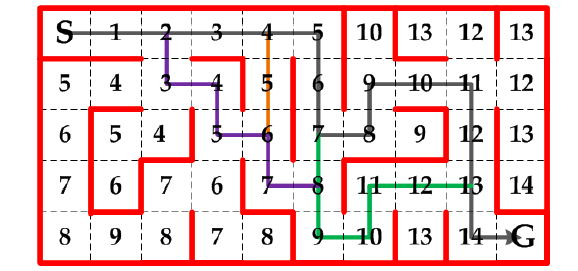
\includegraphics[width=0.8\linewidth]{floodfill.png}
%	\end{center}
%	\centering
%	\small Fonte: adaptado de \citeonline{6734188}
%\end{figure}
Para entender a implementação do algoritmo proposto, as seguintes definições são importantes e deve-se considerar que cada célula do labirinto contenha estrutura de dados para armazenar as seguintes informações:

\begin{enumerate}[leftmargin=2cm,label=\alph*)]
	\item \verb+dist+: esta variável, do tipo inteiro de 16 bits, contém o número de passos para o robô chegar ao alvo;
	\item \verb+wall[4]+: esta variável, na verdade é um vetor do tipo booleano de quatro posições. Cada índice, de 0 a 3, armazena, respectivamente, a informação das paredes descobertas pelo robô ao norte, leste, sul e oeste. Exemplo: \texttt{wall[0]} é 1 quando tem parede ao norte ou 0 quando não tem parede ao norte;
	\item \verb+checked+: esta variável do tipo booleana é alterada para verdadeiro, caso o robô tenha visitado esta célula. Importante para evitar consumo de energia dos sensores de distância e acelerar o robô.
\end{enumerate}


Estas variáveis são acessadas através do identificador da estrutura, de nome \verb+celula+, matriz de 16 $\times$ 16. Cada par de índice $i,j$ da matriz acessa a estrutura correspondente à célula de coordenada (i,j) do labirinto real.
As informações de orientação do robô e suas coordenadas dentro do labirinto também estão armazenadas dentro de uma estrutura de dados, cujo nome é \verb+robo+. As seguintes informações são armazenadas:


\begin{enumerate}[leftmargin=2cm,label=\alph*)]
\item \verb+run+: esta variável terá informação do \emph{status} da corrida. Exemplo: Fazendo uma corrida física ou preparando a volta/ida;
\item \verb+orientacao+: guarda a orientação do robô - NORTE, SUL, LESTE ou OESTE;
\item \verb+sentido_robo+: esta variável armazena o sentido de movimento no momento. Esta informação é dada pelo algoritmo \emph{Flood Fill} sempre antes de adentrar na célula seguinte. Os sentidos são: \verb+FRENTE+, \verb+ESQUERDA+, \verb+DIREITA+ e \verb+VOLTA+;
\item \verb+x+: esta variável armazena a coordenada X em que o robô se posiciona no labirinto;
\item \verb+y+: esta variável armazena a coordenada Y em que o robô se posiciona no labirinto;
\end{enumerate}

A interpretação lógica que abstrai a constituição física do labirinto, pode ser concebida no algoritmo \emph{Flood Fill} como um plano cartesiano, como mostra a Figura \ref{fig:coord}. Cada coordenada é responsável por acessar uma estrutura de dados. A coordenada X representa a linha e a Y representa a coluna da célula. As setas mostram o sentido de crescimento dos números das coordenadas. Também é padronizada a referência de orientação. Ou seja, se o robô está se movimentando da célula (0,0) para a célula (1,0), então ele está andando para o Norte.


Cada célula possui, além da distância, informações das paredes. Por exemplo, na coordenada (15,15) (Figura \ref{fig:coord}), há parede ao norte e ao leste. Então, estas informações podem ser acessadas diretamente da estrutura de dados da célula, ou seja, durante a criação do algoritmo uma estrutura de dados com o nome \verb+celula[16][16]+ foi criado, e desta forma, ao acessar \verb+celula[15][15].wall[NORTE]+ e \verb+celula[15][15].wall[LESTE]+, ambos retornarão verdadeiras, enquanto as variáveis \verb+celula[15][15].wall[OESTE]+ e \verb+celula[15][15].wall[SUL]+ retornarão falsas. Portanto, à medida que o robô vá percorrendo o labirinto, ele vai atualizando as informações das paredes das células, além de atualizar também a variável \verb+checked+, uma variável binária para informação de célula já visitada.



\begin{figure}[!htb]
	\caption{\label{fig:coord}Interpretação do labirinto para o \emph{Flood Fill}}
	\begin{center}
		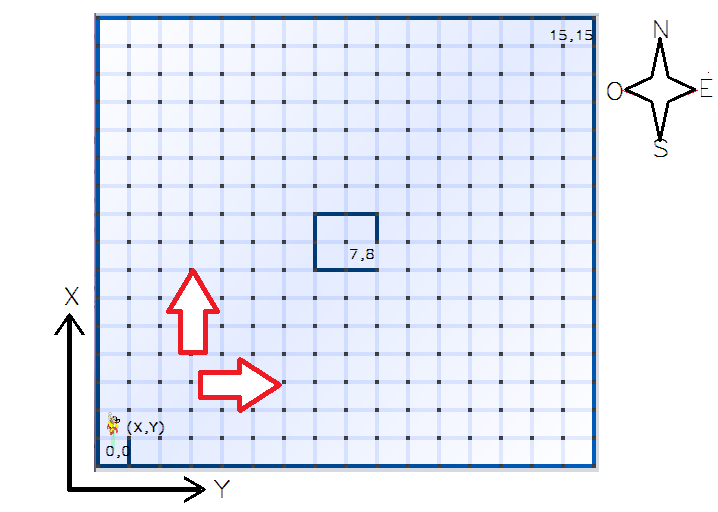
\includegraphics[width=0.7\linewidth]{coord.png}
	\end{center}
	\centering
	\small Fonte: autor (2017)
\end{figure}


O algoritmo enfrenta o labirinto como se ele não tivesse paredes e enumera as células inicialmente conforme mostrado na Figura \ref{fig:dist}. 


\begin{figure}[!htb]
	\caption{\label{fig:dist}Numeração das distâncias sobre o labirinto}
	\begin{center}
		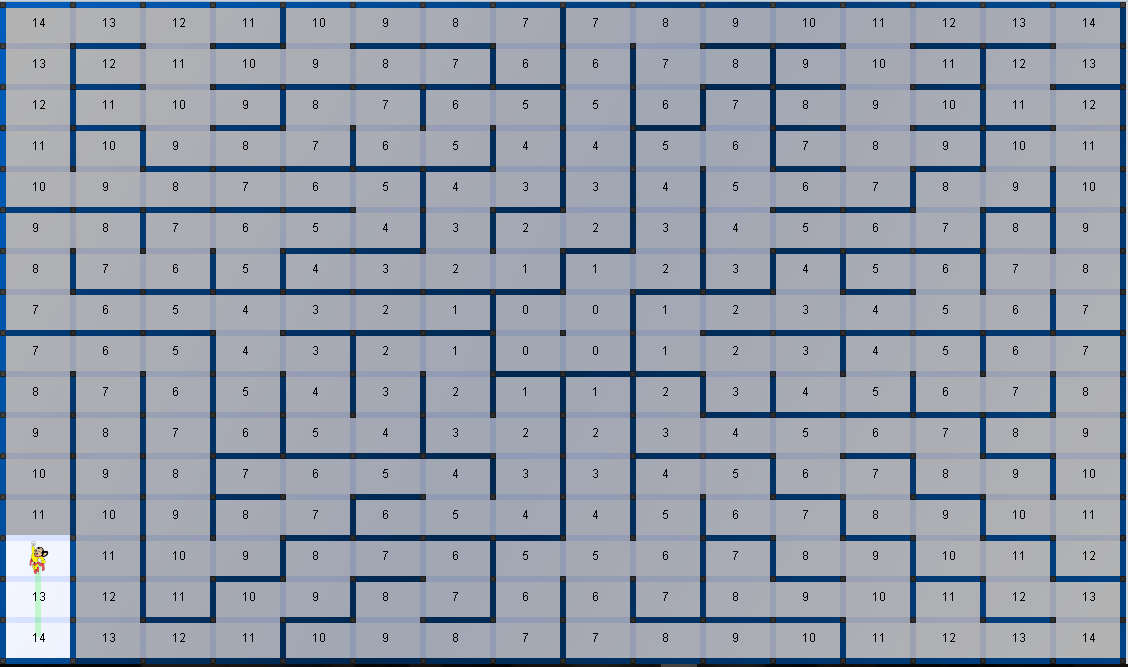
\includegraphics[width=0.7\linewidth]{dist.png}
	\end{center}
	\centering
	\small Fonte: autor (2017)
\end{figure}

Estes valores são o número mínimo de passos até então para chegar ao alvo (valor zero). Na Figura, a parte desconhecida do labirinto pelo robô é mostrado em sombra. Um passo moverá o robô de sua célula atual para a célula com menor distância da célula destino. A princípio, o robô sempre procurará adentrar para a célula que tem o menor valor de distância até encontrar a célula de destino (contém distância zero).



A Figura \ref{fig:diagram1} mostra um algoritmo básico de tomada de decisão. Caso o robô tenha mais de uma opção de percurso, e se um destes percursos envolver a célula à frente e de distância menor que a distância da célula atual, o algoritmo sempre escolherá seguir em frente, visto que para realizar uma curva o robô perde em velocidade, ou seja, o algoritmo tenta ganhar tempo em retas com velocidades maiores. 


\begin{figure}[!htb]
	\caption{\label{fig:diagram1}Fluxograma básico de tomada de decisão}
	\begin{center}
		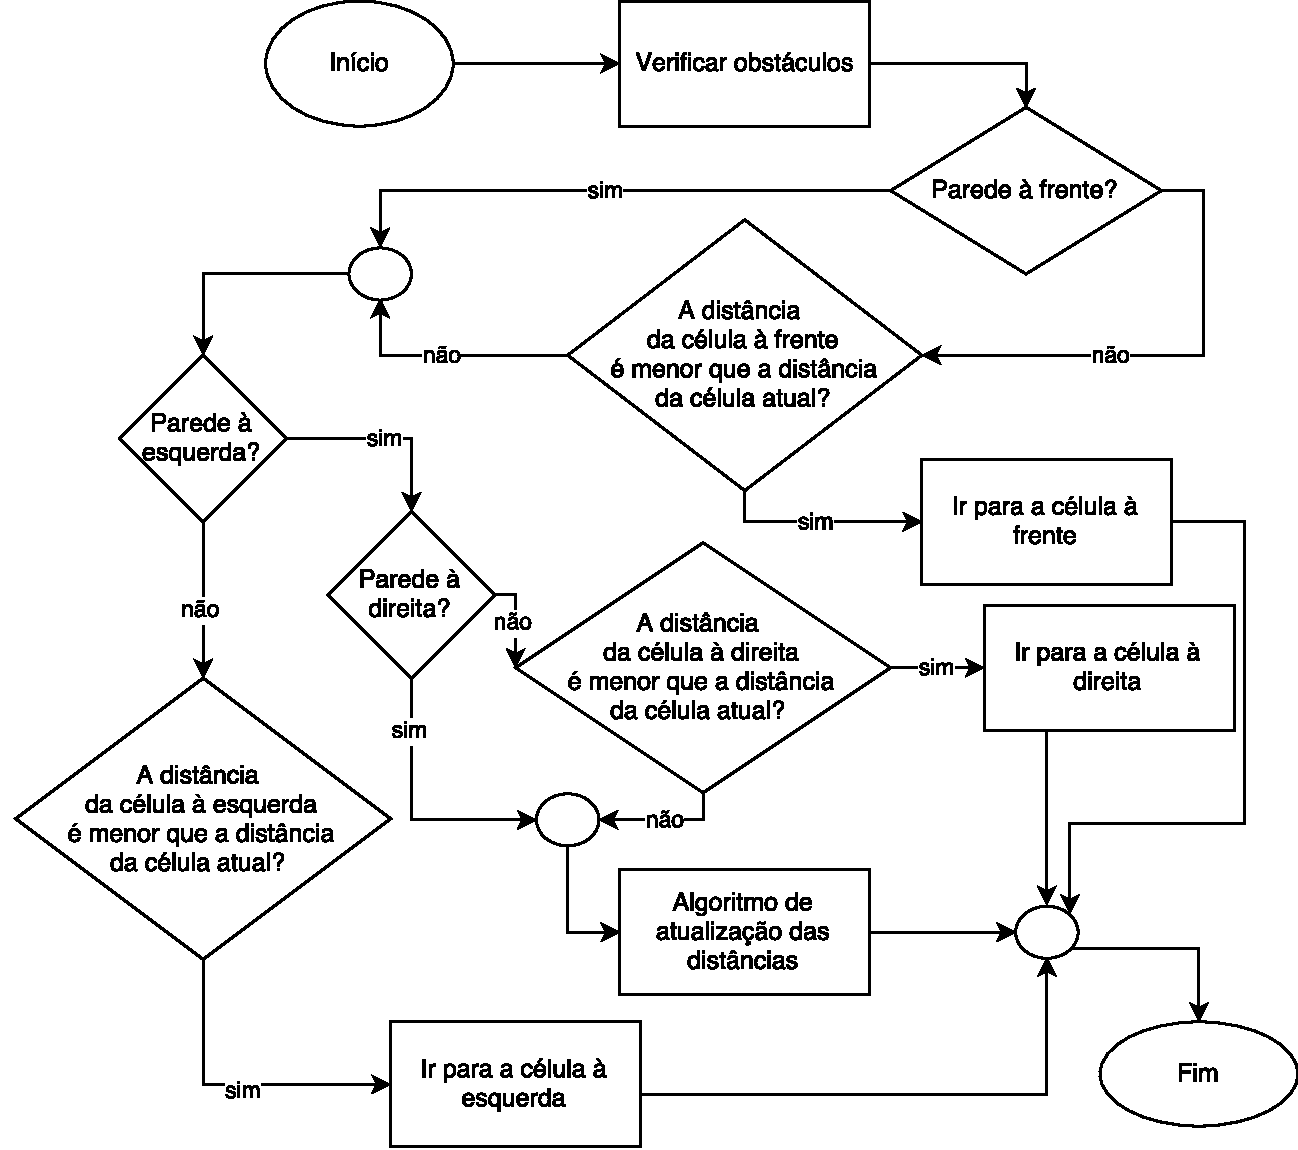
\includegraphics[width=0.9\linewidth]{Diagrama1.pdf}
	\end{center}
	\centering
	\small Fonte: autor (2017)
\end{figure}

%Por exemplo, conforme mostra a Figura \ref{fig:et}, o valor de distância da célula de coordenadas (3,1), por sua vez é acessada por \verb+celula[3][1].dist+, contém valor 3 porque não há conhecimento da parede Leste da célula de coordenadas (2,1) (\verb+celula[2][1].dist+). Até aquele momento, naquela coordenada, o robô seguirá o percurso das setas, uma vez que será o número de passos para chegar ao alvo. Esta concepção é levada para todo o labirinto.

Segundo as regras da competição, as quatro células centrais tem a distância dada como zero. Então a partir destas células, é aplicada a regra das distâncias das células vizinhas para determinar os valores de cada célula.


\subsection{Algoritmo \emph{Flood Fill} não recursivo com otimização de memória}


Neste trabalho o algoritmo \emph{Flood Fill} não recursivo é utilizado como base para desenvolver o esquema de otimização de memória proposto e que tornou mais adequado o seu uso em um \textit{hardware} embarcado e que tenha restrição de memória. À frente mostram-se as discussões sobre a economia de RAM proposto.
%
A seguir é listado o pseudocódigo do algoritmo:
\begin{enumerate}[leftmargin=2cm,label=\alph*)]

\item inicialmente o labirinto é enfrentado como se não existissem paredes;
%First assume that there are no walls
\item enumerar as células com a distância até o alvo, que tem a distância igual a 0;
%Give each cell a distance from the goal. The goal has distance 0.
\item repetir até que se chegue à célula-alvo:
%Repeat until we reach the goal:
	\begin{itemize}[label={--}]
	
	\item ir para a célula vizinha com menor distância;
%Go to the neighboring cell with the smallest distance to the goal
	\item rodar o algoritmo de atualização das distâncias.
%Run the update distances algorithm (see later slide)%
	
	\end{itemize}

\end{enumerate}


O algoritmo \emph{Flood Fill} básico não recursivo é resumido no fluxograma de Figura \ref{fig:diagram2}.


\begin{figure}[!htb]
	\caption{\label{fig:diagram2}Fluxograma básico do \emph{Flood Fill}}
	\begin{center}
		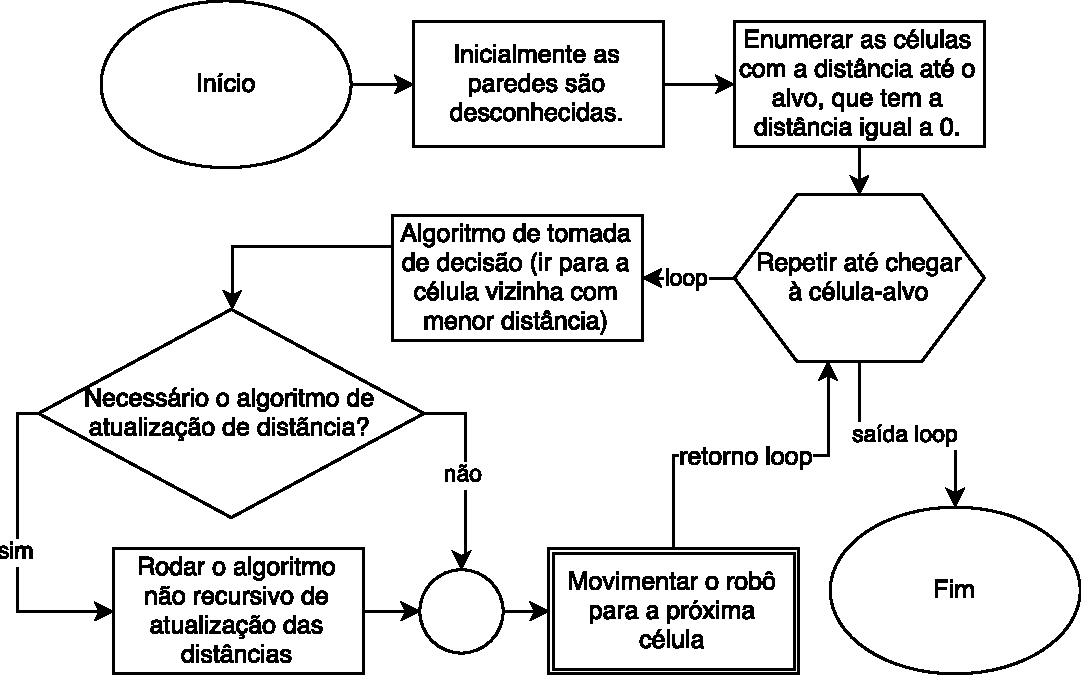
\includegraphics[width=0.8\linewidth]{fluxograma_floodfill.pdf}
	\end{center}
	\centering
	\small Fonte: autor (2017)
\end{figure}




%Each cell has a distance (0-252 for a 16 x 16 maze) and 4 walls (1 bit each). You may also want to have a ?visited? bit for speed runs.
%When you discover a wall, you need to update it in the current cell, and the neighboring cell.
%You can get around this by giving each cell only 2 walls, but you need an extra dummy row/col.
%If you use the ?visited? bit, then you don?t need to run the floodfill update algorithm on cells that you have already visited, meaning you can go faster on them.

O algoritmo de atualização das distâncias não recursivo utiliza pilhas para armazenamento do endereço das células empilhadas. Desta forma, não é necessária a recursividade, que aumentaria o consumo de memória e números de instruções em sistemas embarcados, os deixando lentos.


Os passos necessários para implementar esta parte do algoritmo de atualização, resumida na Figura \ref{fig:diagram3}, estão listados a seguir:

\begin{enumerate}[leftmargin=2cm,label=\alph*)]
\item verificar a pilha se ela está vazia;
%Make sure the stack is empty
\item se alguma parede foi descoberta:
%If there are any new walls discovered
	\begin{itemize}[label={--}]
		\item guardar na pilha a célula atual e as células próximas às paredes.
	\end{itemize}
%Push the current cell and the cells adjacent to the new walls onto the stack
\item enquanto a pilha não esvazia:
	\begin{itemize}[label={--}]
		\item retirar do topo da pilha o endereço da célula guardado
		\item verificar se a distância mínima do vizinho aberto àquela célula + 1 é a distância da célula atual
		\item se isto não é verdade, deve-se modificar o valor da célula atual para o valor mínimo da distância das células vizinhas + 1 e guardar todos os vizinhos abertos para a pilha.
	\end{itemize}
\end{enumerate}

\begin{figure}[!htb]
	\caption{\label{fig:diagram3}Fluxograma básico do algoritmo de atualização das distâncias não recursivo}
	\begin{center}
		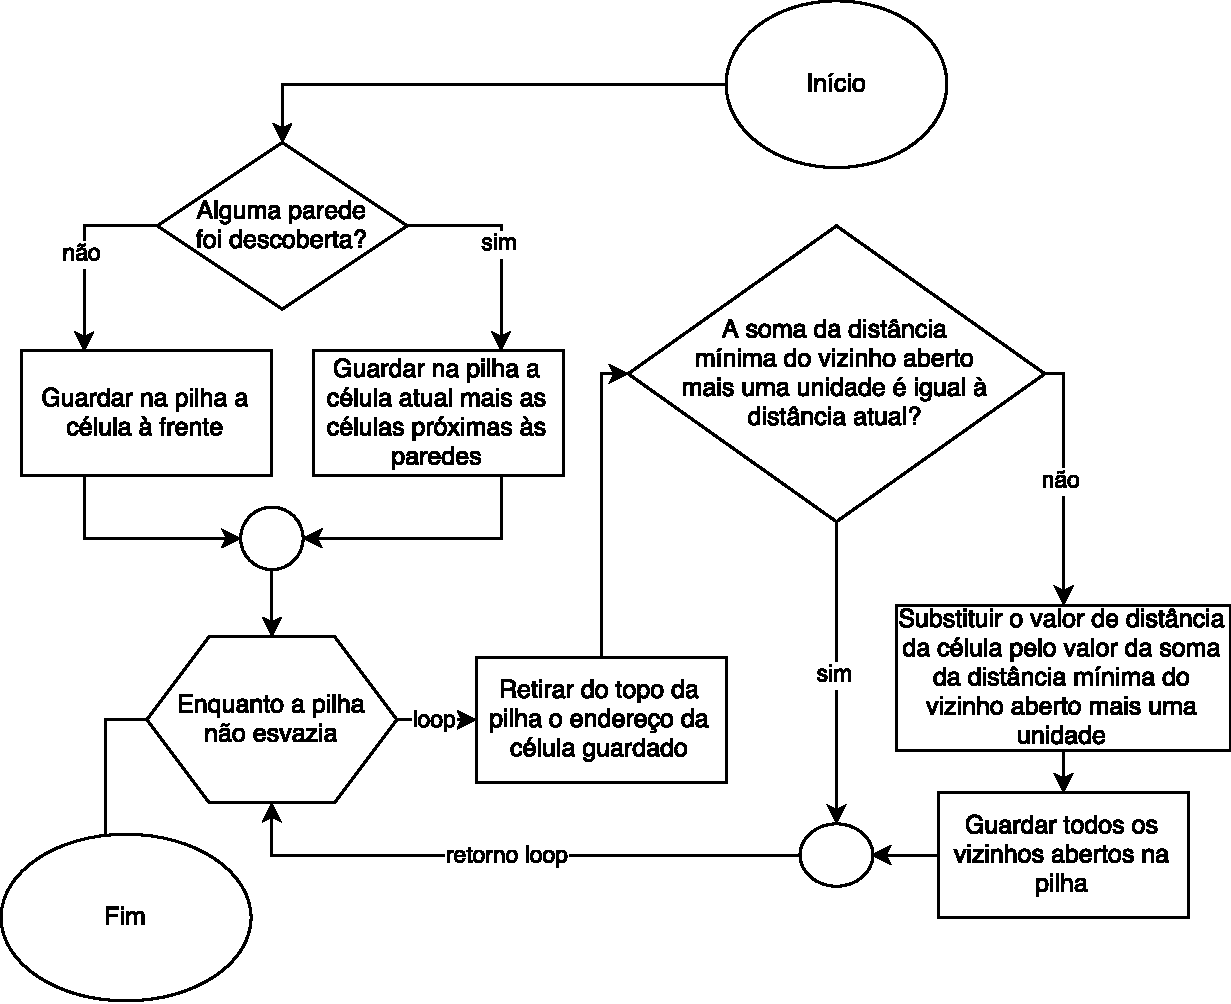
\includegraphics[width=0.8\linewidth]{atualizacao_dist.pdf}
	\end{center}
	\centering
	\small Fonte: autor (2017)
\end{figure}

%While the stack is not empty:
%currCell <- pop the top of the stack
%The distance of currCell should be the minimum open neighbor distance + 1
%If it is not, then set it to that value and push all open neighbors to the stack
%
%\end{enumerate}

O funcionamento do algoritmo inteligente de resolução de labirinto e do algoritmo de atualização das distâncias é melhor entendido através dos exemplos (a), (b) e (c) de Figura \ref{fig:atualiza_dist}.

\begin{figure}[!htb]
	\caption[Exemplo de atualização da distância da célula]{\label{fig:atualiza_dist}Exemplo de atualização da distância da célula}
	\begin{center}
		\subfloat[Exemplo 1]{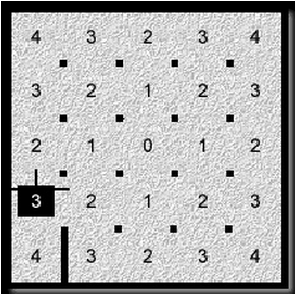
\includegraphics[width=0.3\linewidth]{example_1.png}}
		\hspace*{0.05\linewidth}
		\subfloat[Exemplo 2]{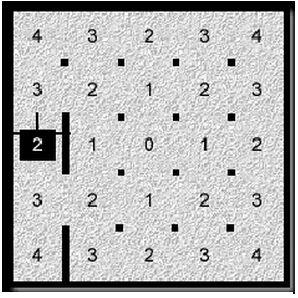
\includegraphics[width=0.3\linewidth]{example_2.png}}
		\hspace*{0.05\linewidth}
		\subfloat[Exemplo 3]{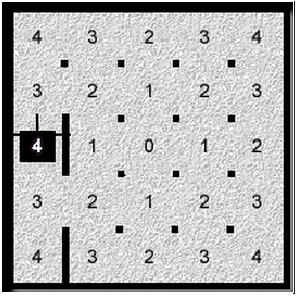
\includegraphics[width=0.3\linewidth]{example_3.png}}
	\end{center}
	\centering
	\small Fonte: autor (2017)
\end{figure}

A Figura \ref{fig:atualiza_dist}(a) mostra a posição inicial do robô, marcado em preto. O labirinto, inicialmente, é desconhecido. O robô tem dois caminhos, mas o robô segue em frente. Ao verificar os obstáculos à frente, na célula seguinte (Figura \ref{fig:atualiza_dist}), o robô atualiza as paredes à leste e à oeste da célula à frente. O próximo passo do algoritmo \emph{Flood Fill} é guardar na pilha as células vizinhas à parede descoberta, ou seja, as células de coordenadas (2,0) e (2,1). Então, até o momento, contém duas células na pilha. Logo em seguida, o algoritmo tira da pilha uma célula e realiza uma comparação da distância entre as células vizinhas à célula recém retirada do topo. Quando existe pelo menos um vizinho aberto à célula retirada do topo, com a distância menor que a distância da célula retirada da pilha, o algoritmo de atualização não realiza alteração da distância e retira uma outra célula da pilha, se houver. No caso da Figura \ref{fig:atualiza_dist}(b), como não há vizinhos abertos com distância menor que 2, então há alteração da distância para o menor valor do vizinho aberto \emph{mais 1}. O valor é alterado para $3 + 1 = 4$, como pode ser visto na Figura \ref{fig:atualiza_dist}(c). Em outras palavras, o robô acaba de descobrir que o caminho não é o ótimo, e altera a distância, de forma a restringir a sua ida pela segunda vez.
	
Desta forma, o robô consegue chegar sempre à célula de destino, de distância zero. Então, como ele volta para a célula de partida e recomeçar uma corrida? A maneira tradicional é a criação de duas estruturas de dados. Uma armazena as distâncias para o robô andar da célula de partida até a célula-destino enquanto a outra estrutura armazena as distâncias calculadas pelo algoritmo para o robô voltar à célula de partida. 
	
Por outro lado, a otimização de RAM é obtida utilizando uma única estrutura de dados para armazenamento das informações das distâncias das células. Após o término da corrida, a célula de distância nula é realocada, ora para a célula de destino, ora para a célula de partida. Então, a partir da célula-alvo de distância nula, é aplicada a regra das distâncias das células vizinhas para determinar os valores de cada célula. Apesar do custo computacional maior em rodar o algoritmo em modo de \emph{varredura} para atualizar as distâncias, nada atrapalha, uma vez que o robô estará parado na célula de valor nulo e o tempo de corrida já fora contabilizado.
	
\subsection{Construindo o algoritmo em linguagem C}
O algoritmo \emph{Flood Fill} é um inteligente solucionador de labirinto. Seu pseudocódigo contém poucas linhas, porém, sua construção é complexa. 

A linguagem escolhida para programar foi a linguagem C, pelo fato de o Micromouse aceitar algoritmos de tal linguagem. Alguns autores programam em outras linguagens e utilizam programas tradutores para linguagem C. Porém, isto não é aconselhável para sistemas embarcados com limitação de memória, uma vez que o programa final torna-se inchado, comprometendo o espaço de memória.

A fim de deixar o código enxuto, utilizou-se do ambiente de desenvolvimento \textit{FALCON C++ IDE}, um programa comum para estudantes de engenharia para desenvolver programas em linguagem C. O programa utiliza como saída de vídeo a janela do \emph{Prompt do Windows} para realizar as impressões através do comando \verb+printf()+.

Frequentemente são utilizados para impressões os símbolos mostados na Figura \ref{fig:simbolos}.


\subsubsection{Máquina de estados para o algoritmo}
A programação torna-se fácil quando se implementa uma \emph{máquina de estados} para códigos extensos. Para tanto, foi criada uma máquina de estados para o algoritmo, com a utilização da função \verb+enum+, função pré-definida em linguagem C para realizar máquinas de estado. 

Logo a seguir constam os estados criados com suas breves funções:
\begin{enumerate}[leftmargin=2cm,label=\alph*)]
	\item \verb+INICIO+: estado responsável para inicializar todas as numerações das células, retirar todas as informações das paredes, dar uma posição, orientação, número da corrida e sentido iniciais para o robô, zerar as variáveis para uso em controle. Após todas as configurações feitas, o algoritmo passa para o próximo estado: \verb+SINAL_PARTIDA+;
	\item \verb+SINAL_PARTIDA+: aguarda o sinal do usuário para sair para a célula-alvo. Lê as informações dos sensores de distância para configurar o próximo estado: \verb+MOVER_ROBO+;
	\item \verb+MOVER_ROBO+: este estado aguarda o robô chegar à entrada da próxima célula. A configuração do próximo estado \verb+VERIFICAR_OBSTACULOS+ é feita após o robô andar uma distância mínima necessária para disparar a leitura das paredes à frente;
	\item \verb+VERIFICAR_OBSTACULOS+: neste estado o robô dispara a leitura dos obstáculos à frente com os sensores IR utilizando a função \verb+getSensoresParede()+ do robô. Este estado é importante e os sensores devem estar calibrados. Uma identificação incorreta das paredes causa falha para definir o próximo sentido e orientação do robô. O algoritmo inteligente de resolução de labirinto \emph{Flood Fill}, representado pelo estado seguinte \verb+DEFINIR_PASSO+, só é executado após o término da leitura das paredes da próxima célula;
	\item \verb+DEFINIR_PASSO+: este é o estado que dispara o algoritmo \emph{Flood Fill}, que indicará o próximo sentido e orientação momentos anteriores à célula frontal. Uma vez definidos, o algoritmo configura o próximo estado: \verb+IMPRIMIR_MAZE+;
	\item \verb+IMPRIMIR_MAZE+: estado responsável por imprimir o labirinto, utilizando os símbolos, e também as coordenadas, estado atual, orientação, sentido, entre outros. O próximo estado é \verb+ESPERAR_CELULA+;
	\item \verb+PREPARA_VOLTA+: este é o estado o qual redefine todas as distâncias das células de tal forma que o robô possa aplicar a regra do \emph{Flood Fill} e retornar à célula de partida. A economia de RAM proposto é feito realizando uma \emph{varredura virtual}, isto é, enquanto o robô aguarda parado o caminho de volta, o algoritmo realiza o percurso virtual de volta. As paredes já conhecidas são utilizadas para atualizar as distâncias das células. Este estado é ativado quando a próxima célula é a \emph{célula de destino};
	\item \verb+PREPARA_IDA+: este é o estado o qual redefine todas as distâncias das células de tal forma que o robô possa aplicar a regra do \emph{Flood Fill} e retornar à célula-alvo. A metodologia para recriar o caminho é a mesma do estado \verb+PREPARA_VOLTA+. Este estado é ativado quando a próxima célula é a \emph{célula de partida};
	\item \verb+ESPERAR_CELULA+: este estado aguarda o robô chegar à próxima célula. O ciclo recomeça no estado \verb+MOVER_ROBO+.
\end{enumerate}

A Figura \ref{fig:estados_robo} mostra os momentos em que há transição de estados durante o percurso do Micromouse no labirinto.

\begin{figure}[!htb]
	\caption{\label{fig:estados_robo}Posição do robô na célula e seus estados}
	\begin{center}
		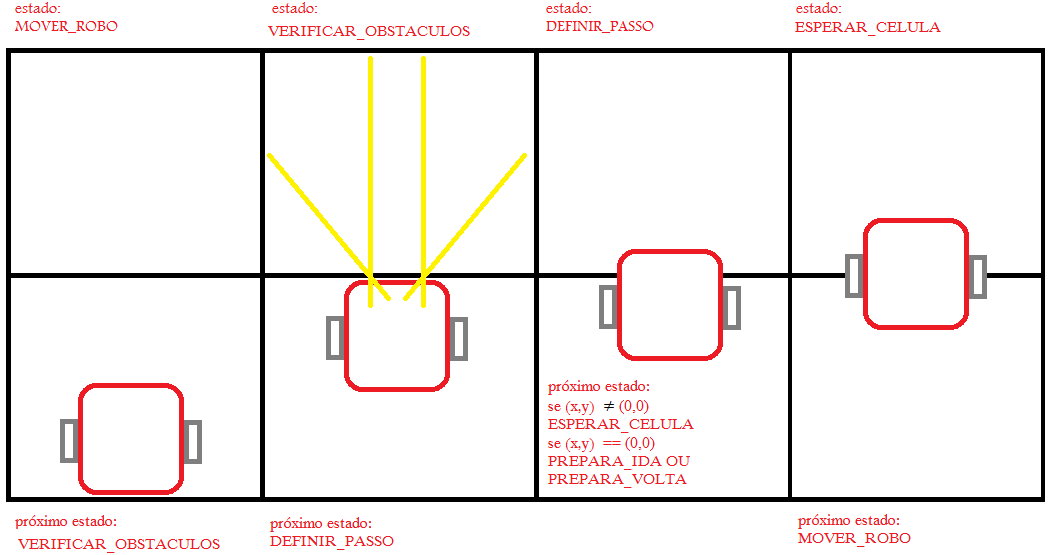
\includegraphics[width=1\linewidth]{estado_robo.png}
	\end{center}
	\centering
	\small Fonte: autor (2017)
\end{figure}

\subsubsection{Funções auxiliares}
O robô em uma célula (x,y) pode tomar quatro direções, a depender dos obstáculos e da tomada de direção do algoritmo Flood Fill. No momento da atualização das paredes em uma célula (x,y), a posição é importante. Algumas funções auxiliares foram criadas para automatizar o processo de atualização e tornar independente da orientação.
	
\begin{enumerate}[leftmargin=2cm,label=\alph*)]
	\item \verb+meia_volta(int i)+: função recebe a orientação atual do robô e retorna a orientação inversa (Ex: Norte - Sul, Leste - Oeste);
	\item \verb+add_x(int orientacao,int x)+: função que ou adiciona uma unidade ao valor x, caso a orientação seja Norte, ou retira uma unidade à coordenada x, caso a orientação seja Sul, ou retorna o mesmo valor x, caso a orientação seja Leste ou Oeste;
	\item \verb+add_y(int orientacao,int y)+: função que adiciona ou retira uma unidade à coordenada y, caso a orientação seja Leste ou Oeste, e retorna o mesmo valor y, caso a orientação seja Norte ou Sul;
	\item \verb+letra_a_esquerda(int i)+: função que recebe a orientação atual do robô e retorna o sentido à esquerda. (Ex: O sentido à esquerda da orientação Leste é Norte; Norte - Oeste; Sul - Leste; Oeste - Sul); 
	\item \verb+letra_a_direita(int i)+: função que recebe a orientação atual do robô e retorna o sentido à direita. (Ex: Norte - Leste; Leste - Sul; entre outros);
	\item \verb+definir_sentido(int orient_ant , int orient_atual)+: esta função é executada após o algoritmo \emph{Flood Fill} e recebe tanto a orientação anterior como a nova orientação. A função compara as duas orientações e retorna um dos quatro estados do movimento do robô: \verb+FRENTE+, \verb+ESQUERDA+, \verb+DIREITA+ ou \verb+VOLTA+. Caso os dois sentidos fossem iguais, o robô continuaria a seguir em frente; Caso uma orientação tenha o sentido contrário da outra, o robô deverá retornar em 180 graus. Se o sentido atual está à esquerda ou à direita em 90 graus de diferença, o robô deverá realizar uma curva de 90 graus. Um novo sentido de movimento é feito próximo à entrada da próxima célula, após a verificação dos obstáculos e execução do algoritmo de resolução \emph{Flood Fill};
	\item \verb+prox_celula_existe(int orientacao, int x, int y)+: esta função recebe como argumentos a orientação atual do robô, e as coordenadas (x,y) e a mesma retorna se a célula existe. Forma simples de verificação quando o robô se encontra nos limites do labirinto, onde não existe na estrutura de dados as células vizinhas.
\end{enumerate}
	

\subsubsection{Função para atualizar as paredes na estrutura de dados}
A função responsável por ler as informações dos sensores infravermelhos e salvar na estrutura da célula, independente da orientação, foi criada. A informação da leitura das paredes é redundante. Ou seja, uma detecção de parede ao norte da célula (1,1), por exemplo, esta informação também deverá ser armazenada na parede Sul da célula (2,1), isto porque a parede divide as duas células. A Figura \ref{fig:estados_robo} mostra o momento do disparo da leitura dos obstáculos, numa posição um pouco à frente da metade da célula. O robô na orientação \texttt{o} e posicionado na coordenada (x,y), recebe e armazena na \verb+struct celula+ corretamente os três bits da função \verb+getSensoresParede()+ conforme os passos a seguir:

\begin{enumerate}[leftmargin=2cm,label=\alph*)]
	\item o bit mais signficativo, representando a leitura do sensor à esquerda do robô, é armazenado na variável \texttt{wall[i]} da célula à frente, onde \texttt{i} é a orientação à oeste da orientação \texttt{o} do robô. Também, na célula oposta à parede recém descoberta, é armazenado o bit, se a célula oposta existir;
	
	\item o segundo bit, representando a leitura dos dois sensores frontais do robô, é armazenado na variável \texttt{wall[o]} da célula à frente, onde \texttt{o} é a própria orientação do robô. Também na célula oposta à parede recém descoberta, é armazenado o bit, se a célula oposta existir;
	
	\item o bit menos signficativo, representando a leitura do sensor à direita do robô, é armazenado na variável \texttt{wall[i]} da célula à frente, onde \texttt{i} é a orientação à leste da orientação \texttt{o} do robô. Também, na célula oposta à parede recém descoberta, é armazenado o bit, se a célula oposta existir;
	
	\item as \emph{funções auxiliares} ajudam a automatizar todo o processo anteriormente, para qualquer que seja a orientação do robô e posição do mesmo no labirinto;
	
	\item se a célula já foi visitada, ou seja, se \verb+celula[add_x(o,x)][add_y(o,y)].checked+ é \textbf{verdadeiro}, os sensores não são utilizados.
\end{enumerate}


\subsubsection{Inicializando as distâncias das células para o alvo no centro do labirinto }
A enumeração inicial das distâncias, conforme é mostrada na Figura \ref{fig:dist}, é feita pelo trecho do código da função \verb+inicializa_lab()+. Nesta mesma função, o \emph{check} de cada célula é zerada. Este trecho também faz parte da função \verb+a_todo_vapor()+, que só é executado no estado \verb+PREPARA_IDA+, que por sua vez, é responsável por reiniciar as distâncias e executar o \emph{Flood Fill} no \emph{modo de varredura} utilizando somente uma estrutura de dados para armazenamento das distâncias das células.
	
%$\vdots$
%\begin{verbatim}
%int i=0;
%int j=0;
%//i => linha ; j=> coluna
%
%for(i=0;i<16;i++){
%    for(j=0;j<16;j++){
%        //Zerando a variável booleana check
%        celula[i][j].checked = 0;
%        
%        //enumerando as células
%        if(j<8 && i<8){
%            celula[i][j].dist = 14 - j - i;
%        }
%        else if(i<8 && j>=8){
%            celula[i][j].dist = j - i - 1;
%        }
%        else if(j<8){
%            celula[i][j].dist = i - j  - 1;
%        }
%        else{
%            celula[i][j].dist = j + i - 16 ;
%        }
%    }
%}
%\end{verbatim}
%$\vdots$

\subsubsection{Reinicializando as distâncias das células quando o alvo é realocado para a célula de partida }
A automação da enumeração das distâncias, para permitir ao robô voltar à célula de partida, é feita pelo trecho do código da função \verb+a_volta_do_robo()+. Esta função é executada somente no estado \verb+PREPARA_VOLTA+, o qual realiza a preparação da volta após êxito na corrida de ida. No mesmo código, as paredes-vértices das quatro células nulas também são consideradas, atualizando os bits das paredes correspondentes nas estruturas das células, exceto para a célula de chegada (x,y). Segundo as regras para competição, há somente uma entrada para as células centrais. Da mesma forma para o estado \verb+PREPARA_IDA+, o procedimento é feito para o estado \verb+PREPARA_VOLTA+, que por sua vez, é responsável por reiniciar as distâncias e executar o \emph{Flood Fill} no \emph{modo de varredura} utilizando somente uma estrutura de dados para armazenamento das distâncias das células.

%$\vdots$
%\begin{verbatim}
%for(i=0;i<16;i++){
%    for(j=0;j<16;j++){
%		
%	  // enumerando as células para voltar
%      celula[i][j].dist = i+j;
%      if(i>6 && i<9 && j>6 && j<9)
%      {	
%    	if(i!=robo.x || j!=robo.y){
%        
%            if(i==7){
%        	    //quadrante inferior
%        	    celula[i][j].wall[SUL] = 1;
%        	    celula[i-1][j].wall[NORTE] = 1;
%            }else
%            {
%            	//quadrante superior
%            	celula[i][j].wall[NORTE] = 1;
%        	    celula[i+1][j].wall[SUL] = 1;
%            }
%        
%            if(j==7){
%        	    //quadrante esquerdo
%        	    celula[i][j].wall[OESTE] = 1;
%        	    celula[i][j-1].wall[LESTE] = 1;
%        	
%            }else
%            {
%        	    //quadrante direito
%        	    celula[i][j].wall[LESTE] = 1;
%        	    celula[i][j+1].wall[OESTE] = 1;
%            }
%    	}
%      }
%    }
%}
%\end{verbatim}
%$\vdots$

\subsubsection{Algoritmo Flood Fill em C}
Esta é a parte mais importante de todas. O algoritmo \emph{Flood Fill} é a parte inteligente, porque quando ele é executado (no final de cada célula), o mesmo retorna uma nova orientação e sentido para o robô, sendo o guia virtual do robô. Esta parte do programa integra o algoritmo de tomada de decisão (fluxograma na Figura \ref{fig:diagram1}), e o algoritmo de atualização das distâncias (fluxograma na Figura \ref{fig:diagram2}). Uma função de nome \verb+floodfill()+ foi criada para realizar todo o processo necessário.

A estrutura de dados bastante utilizada nesta função é a Pilha, que na literatura é conhecido como LIFO (último a entrar e primeiro a sair). Ela tem como função ser memória temporária para dados, registradores ou tarefas, onde os itens são incluídos e retirados da mesma extremidade da lista. O algoritmo \emph{Flood Fill} armazena em estrutura de dados do tipo PILHA os endereços das células. As seguintes funções para acesso à Pilha foram criadas:

\begin{enumerate}[leftmargin=2cm,label=\alph*)]
\item \verb+Pilha_Construtor()+: responsável por zerar a contagem de empilhamentos e configurar o topo como NULO. Esta função é executada no estado \verb+INICIO+;
\item \verb+Pilha_Tamanho()+: responsável por retornar o número de empilhamentos;
\item \verb+Pilha_Vazia()+: retorna \emph{verdadeiro}, caso não tenha nenhum endereço na pilha;
\item \verb+Pilha_Push(CELULA *point)+: recebe o endereço da célula via argumento, aloca um espaço na RAM dinamicamente e guarda o valor do endereço no topo da pilha;
\item \verb+*Pilha_Pop()+: retira do topo da pilha o endereço da célula empilhada e retorna o endereço para um ponteiro do tipo \verb+struct+.
\end{enumerate}

O algoritmo é executado após a verificação dos obstáculos à frente. De acordo com o fluxograma do algoritmo, Figura \ref{fig:diagram2}, são empilhadas somente as células próximas às paredes recém descobertas. 

%O trecho mostra esta parte:
%
%$\vdots$
%\begin{verbatim}
%  CELULA *C; // Ponteiro para resgatar o endereço da célula
%  // guardada no topo da pilha
%  int i,value,update,k,x,y,od,oe; //Variáveis auxiliares
%  k=0;
%  update=0;
%  
%  x = add_x(robo.orientacao,robo.x);
%  y = add_y(robo.orientacao,robo.y);
%  od = letra_a_direita(robo.orientacao);
%  oe = letra_a_esquerda(robo.orientacao);
%   
%  //Toda vez que encontra parede nova ou quando a pilha está vazia
%  //adicionar a célula próxima à pilha. 
%  //Esta é a regra número 1 do flood fill.
%  if(news_walls || Pilha_Vazia()){
%    //adcionei a célula seguinte à pilha para análise da trajetória
%    //Pseudocódigo diz que é preciso adicionar à pilha a célula seguinte
%    //quando existem obstáculos
%    if(robo.run != 16)
%    {
%      //à esquerda
%      if((news_walls & 0b100) == 0b100)
%        if(prox_celula_existe(oe, x, y))
%        {
%          Pilha_Push(&celula[add_x(oe,x)][add_y(oe,y)]);
%        }
%      //à direita   
%      if((news_walls & 0b001) == 0b001)
%        if(prox_celula_existe(od, x, y))
%        {
%          Pilha_Push(&celula[add_x(od,x)][add_y(od,y)]);
%        }
%      //à frente
%      if((news_walls & 0b010) == 0b010)
%        if(prox_celula_existe(robo.orientacao, x, y))
%        {
%          Pilha_Push(&celula[add_x(robo.orientacao,x)][add_y(robo.orientacao,y)]);
%        }
%    }
%    
%    //Sempre colocar a célula a entrar por último, neste caso.
%    Pilha_Push(&celula[x][y]);
%}
%\end{verbatim}
%$\vdots$

Após isto, o topo da pilha é retirado e representa a célula a entrar. O acesso às variáveis da estrutura da célula é feito por meio do \emph{ponteiro}. Um ponteiro \verb+C+, do mesmo tipo da estrutura de dados \verb+struct+, é criado para receber o endereço. São feitas as análises de vizinhança para tomada de decisão a partir da célula de endereço armazenado no ponteiro.
%
%$\vdots$
%\begin{verbatim}
%// Essa parte procura caminhos à frente.
%// Se UMA das células vizinhas tiver o valor de distância +1 igual
%// ao valor da célula central, então não é necessário atualizar
%// o valor da célula central. Regra número 3 do flood fill.
%
%k=0;
%for(i=0;i<4;i++){
% if(C->wall[i]==0){
%  //PAREDE LIVRE NO SENTIDO i da célula seguinte.
%  //Contabilizando o número de vizinhos abertos
%  if(((celula[add_x(i,C->ii)][add_y(i,C->jj)].dist)+1)==C->dist)
%  {
%   //Tem um vizinho aberto!!!
%   k++;
%  }
%  if(value>(celula[add_x(i,C->ii)][add_y(i,C->jj)].dist))
%  {
%   //Caçar uma vizinhança aberta com a menor distância.
%   value = celula[add_x(i,C->ii)][add_y(i,C->jj)].dist;
%   
%  }
% }
%}
%\end{verbatim}
%$\vdots$

	Se há um vizinho aberto, uma variável auxiliar \verb+k+ não será contabilizada. Sendo nula, o algoritmo de atualização das distâncias é ignorado e o programa retira um novo endereço da pilha, caso a função \verb+Pilha_vazia()+ retorne falso. Caso contrário, o algoritmo \emph{Flood Fill} é encerrado.
	
	Após todo o processo \emph{Flood Fill}, são definidos uma nova orientação e um novo sentido, isto para as células de distância não nula. O trecho do código, que realiza a escolha da orientação e sentido de forma automática, está logo a seguir:
	
\begin{enumerate}[leftmargin=2cm,label=\alph*)]
	\item se a próxima célula não é a célula-destino, e se não houver parede e sua distância é menor que a da célula atual, o robô continuará com o mesmo sentido;
	\item caso contrário, procurar vizinhanças abertas com distância menor que a distância da célula atual, sendo que a nova orientação será o mesmo sentido do vizinho aberto;
	\item por último, o algoritmo configura as coordenadas do robô para as da próxima célula.
\end{enumerate}

Portanto, o algoritmo proposto tomou forma e seus resultados são comentados no próximo capítulo.
%
%\begin{verbatim}
%//proxima célula não é o alvo, então definir a nova orientação
%if(celula[robo.aux[1]][robo.aux[2]].dist)
%{
% //Agora é a etapa que define a orientação e o passo final do robô.
% if(celula[robo.aux[1]][robo.aux[2]].wall[robo.aux[0]]==0 && 
% ((celula[add_x(robo.aux[0],robo.aux[1])][add_y(robo.aux[0],robo.aux[2])].dist)+1)
% ==celula[robo.aux[1]][robo.aux[2]].dist)
% {
%  //Se não existir parede na célula seguinte que impeça que o robô siga com 
%  //a mesma orientação anterior... Ele vai continuar com a mesma orientação
%  //(ganha em velocidade, porque ele não vai precisar diminuir na curva.)
%  
%  robo.sentido_robo = FRENTE;  // Ou seja, seguir em frente
%  robo.orientacao = robo.aux[0];  // Continuar com a mesma orientação
%  
% }else{
%  //Caso contrário, ele vai procurar a orientação certa
%  for(i=0;i<4;i++){
%   if(celula[robo.aux[1]][robo.aux[2]].wall[i]==0){
%    //Se o valor da célula a frente do robô for igual ao valor da célula do
%    //robô atual +1, então ele vai pra esse sentido
%    //já que todas as células foram atualizadas.  
%    if(((celula[add_x(i,robo.aux[1])][add_y(i,robo.aux[2])].dist)+1)
%    ==celula[robo.aux[1]][robo.aux[2]].dist)
%    {
%     // Definir sentido 
%     //0 - FRENTE
%     //1 - ESQUERDA
%     //2 - DIREITA
%     //3 - VOLTA
%     
%     definir_sentido(robo.aux[0], i);
%     robo.orientacao = i;
%     //Atualizar as coordenadas para a célula seguinte
%     // robo.x = robo.aux[1];
%     // robo.y = robo.aux[2];
%     break;
%    }
%   }
%  }
% }
%//Indicar o próximo estado do algoritmo
%nextState = IMPRIMIR_MAZE;
%}
%\end{verbatim}

\section{Controle}
Para o correto entendimento da implementação do controle digital no Micromouse, um pequeno histórico dos controladores de processos é mostrado à frente.


\subsection{Histórico}

Com o rápido desenvolvimento dos computadores digitais e sua larga aplicação na engenharia, a identificação de modelos discretos foi amplamente desenvolvida e empregada em diversas áreas do conhecimento \cite{demodelo}. O Método dos Mínimos Quadrados estima os parâmetros de um modelo de equação discreta para qualquer processo, e as equações podem ser usadas para simulações de controladores diversos.

Karl Friedrich Gauss formulou o \emph{Princípio dos Mínimos Quadrados} ao final do século 18 para prever as trajetórias de planetas e cometas a partir das observações realizadas. K. F. Gauss estabeleceu que os parâmetros desconhecidos de um modelo matemático deveriam ser selecionados de modo que:

\begin{citacao}
o valor mais provável das grandezas desconhecidas é a quantidade que minimiza a soma dos quadrados da diferença entre os valores atualmente observados e os valores calculados multiplicados por números que medem o grau de precisão, onde quanto mais precisa a medida, maior sua ponderação. \apud[p.-123]{LJUNG:1983}{COELHO:2015}.
\end{citacao}


Em 1920, Foxboro introduziu um controlador baseado em ar comprimido com ação integral. Em um dado momento as empresas de sensores introduziram instrumentos e controladores que poderiam implementar controladores PID. Embora Maxwell e Routh tenham desenvolvido uma base matemática para assegurar a estabilidade de um sistema realimentado, o projeto de controladores era baseado na experiência do projetista e em tentativa e erro. Dispositivo PID é composto por: um termo Proporcional para fechar a malha de realimentação, um termo Integral para garantir erro nulo à referência constante e às entradas de perturbação, e um termo Derivativo para melhorar a estabilidade e a boa resposta dinâmica. Como parte da evolução do projeto do controlador PID, um passo importante para sintonizar controladores deste tipo foi dado em 1942, quando Ziegler e Nichols, que trabalhavam para Taylor Instruments, publicaram o seu método de sintonia com base em dados experimentais \cite{FRANKLIN:2013}.

\begin{citacao}
	Partindo do controle proporcional realimentado, o primeiros engenheiros descobriram a ação de controle integral como forma de eliminar o erro em regime permanente. Entretanto, encontravam, em muitos casos, uma resposta dinâmica pobre; assim, um termo de "antecipação" baseado na derivada foi adicionado. \cite[p. -160]{FRANKLIN:2013}
\end{citacao}

\begin{figure}[!h]
	\caption{\label{fig:block_pid}Diagrama de blocos do controle PID em malha fechada}
	\begin{center}
		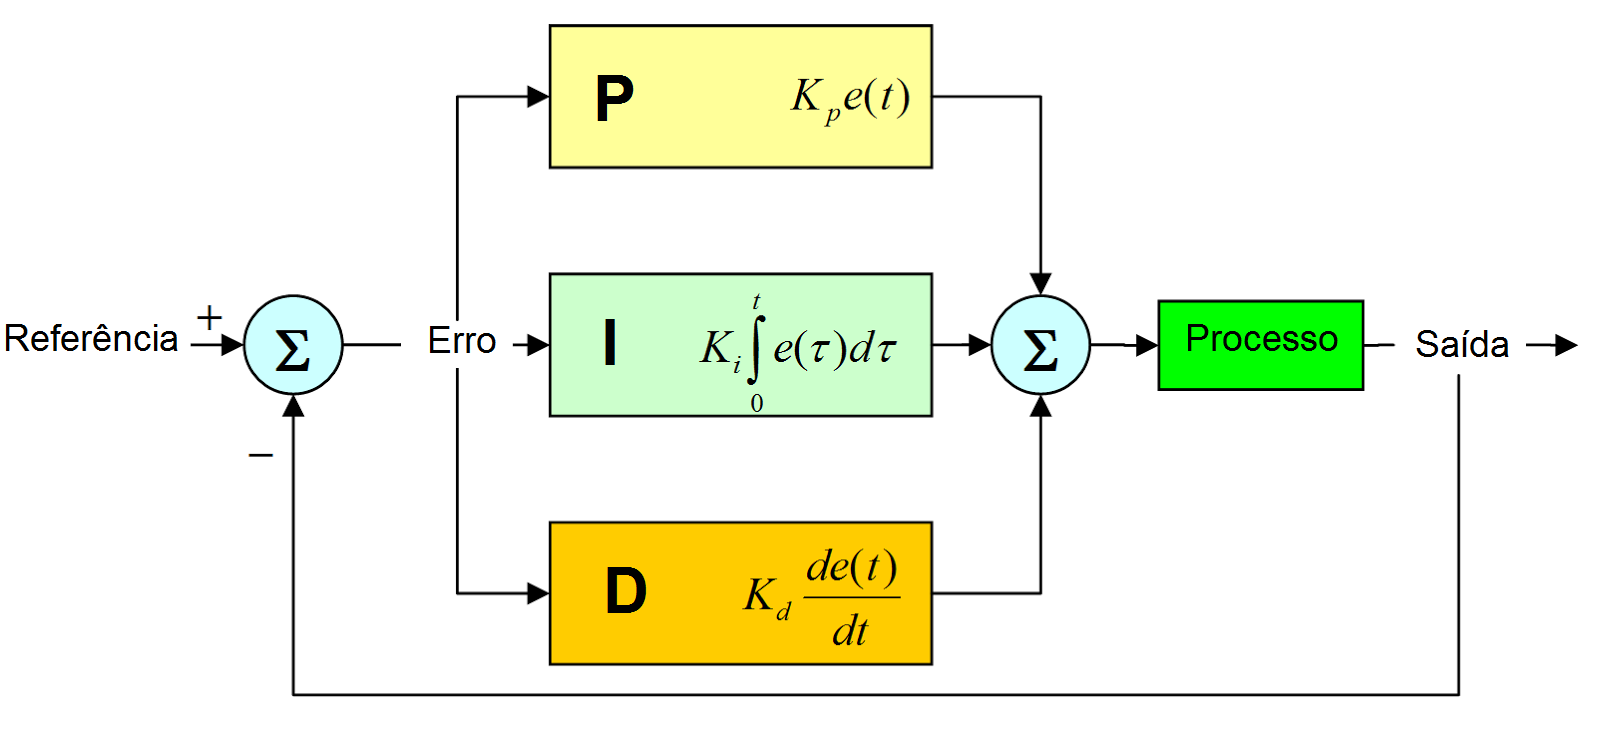
\includegraphics[width=.9\linewidth]{pid_2.png}
	\end{center}
	\legend{Fonte: autor (2017)}
\end{figure}

O resultado destes três controladores tem nome: controlador de três termos, ou PID, e tem a função de transferência (\ref{eq:pid}), sendo $k_P$ o termo proporcional, $k_I$ o termo integral e $k_D$ o termo derivativo. A Figura \ref{fig:block_pid} mostra o diagrama de blocos do sistema em malha fechada.


\begin{equation}
	\label{eq:pid}
	\begin{split}
	G_c(s) 	&=	k_p + k_I/s + (k_D)s
	\end{split}
\end{equation}
	
Os experimentos com relé na malha de realimentação (Figura \ref{fig:rele_malha}), com o propósito de identificação de processos, tornaram-se populares a partir do trabalho de \.{A}str\"{o}m e H\"{a}gglund (1984). Este método foi utilizado para determinar o ganho crítico e a frequência crítica e, por consequência automatizar o método de oscilação de projeto do controlador PID proposto por Ziegler e Nichols (1942). A abordagem baseia-se na modelagem da não linearidade através de sua função descritiva e na interpretação em termos do diagrama de \emph{Nyquist} para a obtenção de informação em frequência do processo. A identificação do processo é feita a partir da estimação em frequência da função de transferência do processo num experimento de malha fechada \cite{COELHO:2015}.

\begin{figure}[!h]
	\caption{\label{fig:rele_malha}Relé na malha realimentada}
	\begin{center}
		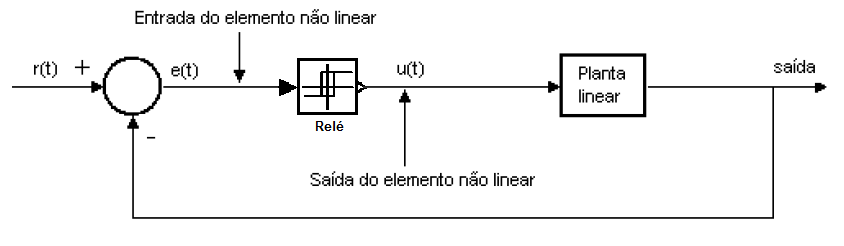
\includegraphics[width=.9\linewidth]{rele.png}
	\end{center}
	\legend{Fonte: adaptado de \citeonline{de2004auto}}
\end{figure}

	\subsection{Determinando o tempo de amostragem do processo}
	Em qualquer processo é importante o conhecimento dos limites da planta em \emph{malha aberta} ou em \emph{malha fechada} para determinar o tempo de amostragem do sistema. A técnica para a escolha do tempo de amostragem para sistemas de controle digitais, segundo \citeonline{LANDAU:2006}, é o cálculo a partir da largura de banda do sistema em malha fechada ou estimá-la a partir da resposta ao degrau. A regra usada para a escolha do tempo de amostragem é mostrado em (\ref{eq:ts}), onde $f_s$ é a frequência de amostragem e ${f_B}^{CL}$ é a largura de banda do sistema de malha fechada. A regra da Equação (\ref{eq:ts}) é usada igualmente em malha aberta, realizando a estimação da largura de banda do processo e substituindo-a por ${f_B}^{CL}$. Desta forma, em malha aberta, o tempo de amostragem pode ser calculada de $1/5$ a $1/10$ do tempo de assentamento da resposta ao degrau.

\begin{equation}
	\label{eq:ts}
	\begin{split}
	f_s 	&=	(6~a~25){f_B}^{CL}
	\end{split}
\end{equation}	

Como a entrada do sistema \textit{encoder}-rodas é um sinal PWM com \emph{duty} entre 0 e 100 \%, para este teste, programou-se um \emph{duty cicle} de 100\% para um tempo de amostragem inicial de $1~ms$ e a saída do processo estabilizou em $T_{assent} = 100~ms$, como pode ser observado na Figura \ref{fig:malha_aberta_dc}.


\begin{figure}[!htb]
	\caption{\label{fig:malha_aberta_dc}Sistema Motor-\textit{encoder} em malha aberta}
	\begin{center}
		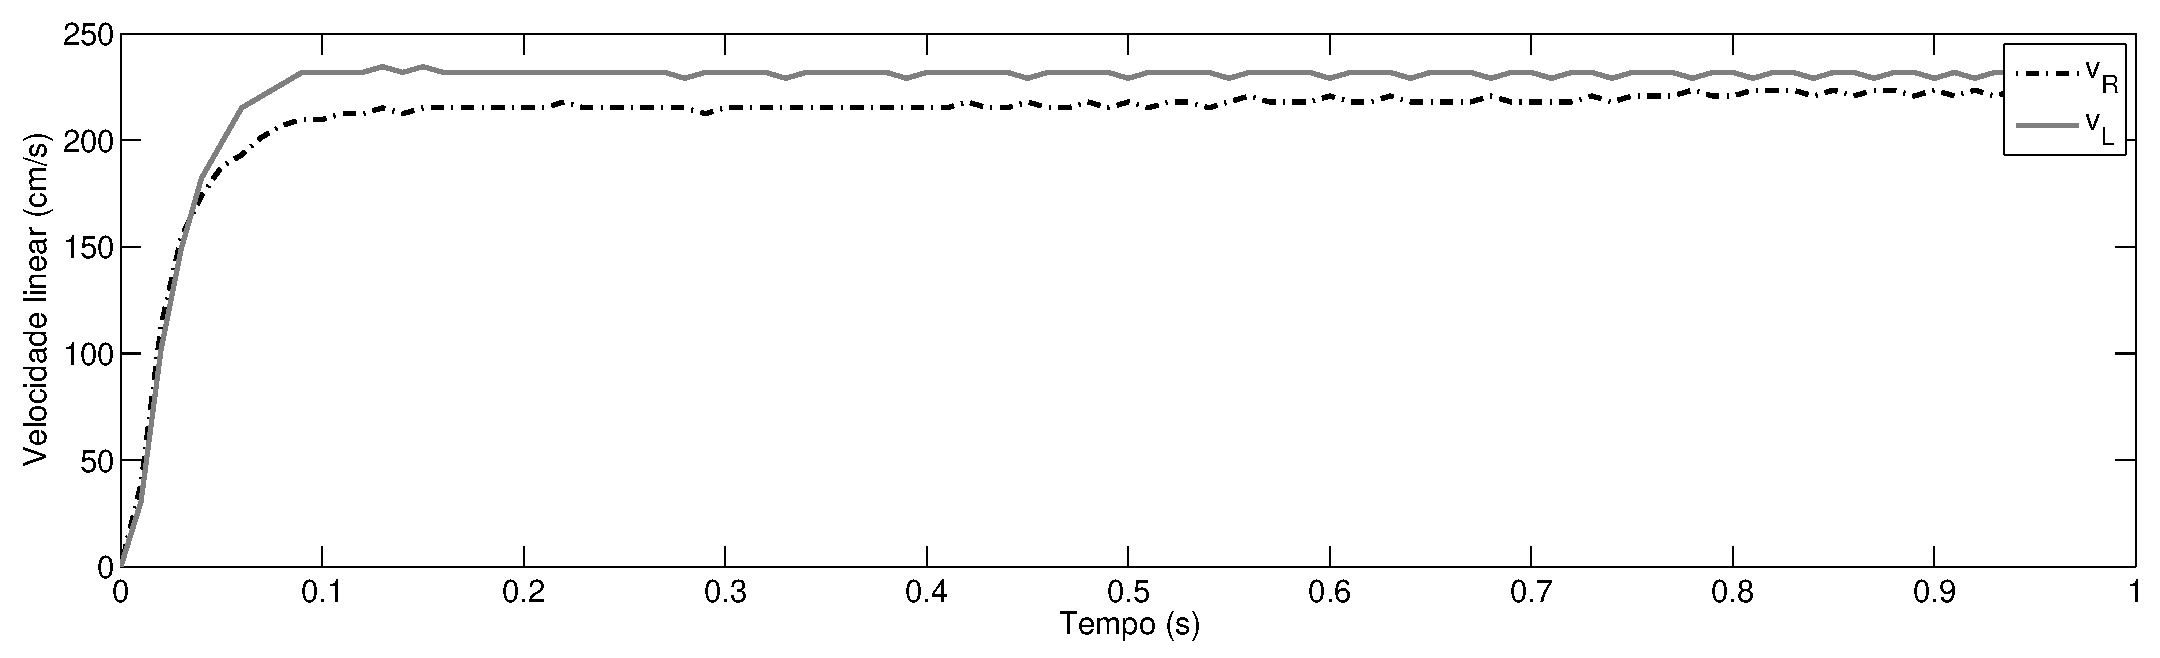
\includegraphics[width=.9\linewidth]{resp_malha_aberta.eps}
	\end{center}
	\legend{Fonte: autor (2017)}
\end{figure}

	
	\citeonline{LANDAU:2006} disponibilizou alguns períodos de amostragem de diferentes processos para controle digital. A Tabela \ref{tab:ts_plants} mostra para cada tipo de planta faixas de tempos de amostragem ideais. Como o processo do Micromouse é composto basicamente por motores DC, a escolha de $~10ms$ para o tempo de amostragem torna-se adequada. Portanto, o tempo de amostragem adotado para o sistema de controle digital do Micromouse é de $T_s = ~10ms$, considerando $T_{assent}/10$.
	
\begin{table}[!htb]
\centering
\caption{\label{tab:ts_plants}Escolha do tempo de amostragem para sistemas de controle}


	\begin{tabular}{c|c}
	\textbf{Tipo de variável (ou planta)} & \textbf{Tempo de Amostragem (s)} \\ 
	\hline 
	\textbf{Vazão} & 1 - 3 \\ 
	\hline 
	\textbf{Nível} & 5 - 10 \\ 
	\hline 
	\textbf{Pressão} & 1 - 5 \\ 
	\hline 
	\textbf{Temperatura} & 10 - 180 \\ 
	\hline 
	\textbf{Destilação} & 10 - 180 \\ 
	\hline 
	\textbf{Motores DC} & 0,001 - 0,05 \\ 
	\hline 
	\textbf{Catalystic reactors} & 10 - 45 \\ 
	\end{tabular} 
\legend{Fonte: adaptado de \citeonline[p. 31--32]{LANDAU:2006}}
\end{table}
	
	
	\subsection{Sintonia via Método do Relé}
	O controle PID geralmente é conhecido como um controle clássico para processos SISO (única entrada e única saída). Portanto, existem muitas pesquisas sobre métodos de ajuste do controle PID para o sistema SISO.
	O controlador adaptativo com autossintonia, do tipo \emph{auto-tunning}, insere um relé no contexto da estimação de modelos matemáticos de ordem reduzida a partir da resposta em frequência. Segundo \citeonline{COELHO:2015}, na atualidade, é inevitável uma breve descrição da metodologia do relé no contexto da estimação de modelos matemáticos de ordem reduzida a partir da resposta em frequência.
	O método do relé na malha de realimentação, como já foi dito anteriormente, tem o propósito de descobrir o ganho crítico e a frequência crítica.
	
	Controladores PID (proporcional, integral e derivativo) são os controladores lineares mais utilizados na prática. O ajuste de seus parâmetros é um dos problemas de controle mais considerados. Para o caso de plantas de modelo desconhecido, \.{A}str\"{o}m apresentou um método de auto-ajuste de parâmetros de PID utilizando um elemento não linear. Tendo dado ênfase ao uso do relé ideal, \.{A}str\"{o}m sugeriu como extensão à possibilidade do uso do relé com histerese com o objetivo de melhorar a relação sinal-ruído, embora não tenha apresentado um algoritmo de auto-ajuste correspondente.
	
	\.{A}str\"{o}m propôs um sistema de sintonia automática de controle PID. Este método utiliza o método da linearização harmônica com base no conceito da função descritiva para estimar parâmetros do sistema.
	
%\begin{figure}[!h]
%	\caption{\label{fig:reles}Relé sem histerese (à esquerda) e Relé com histerese (à direita)}
%	\begin{center}
%		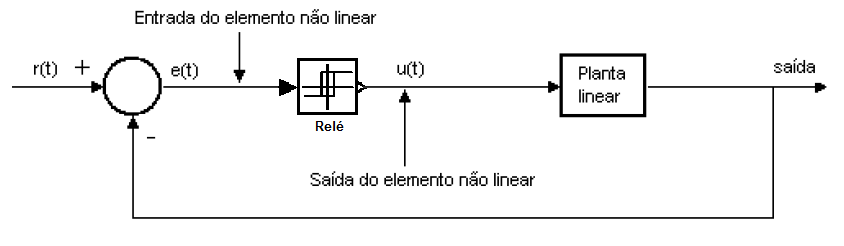
\includegraphics[width=.9\linewidth]{rele.pdf}
%	\end{center}
%	\legend{Fonte: \cite{COELHO:2015}}
%\end{figure}

\begin{figure}[!htb]
	%\caption[Percurso do robô no labirinto \emph{Seoul} - primeira corrida \emph{real}]{\label{fig:ModelagemLab2}Percurso do robô no labirinto Seoul}
	\caption{\label{fig:reles}Relé - elemento não linear}	
	\begin{center}
		\subfloat[Relé sem histerese]{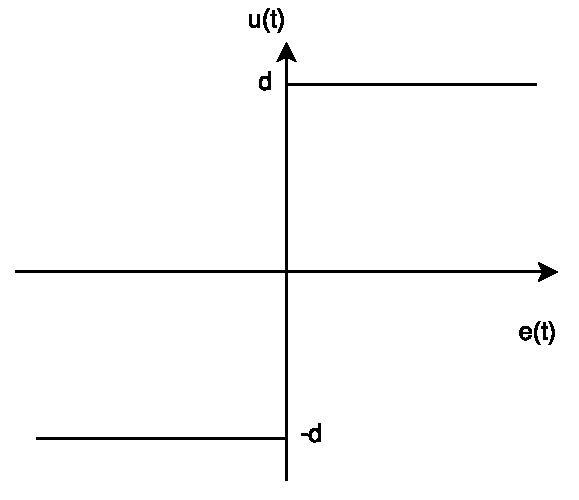
\includegraphics[width=0.4\linewidth]{rele_sem_hist.pdf}}
		\hspace*{0.1\linewidth}
		\subfloat[Relé com histerese]{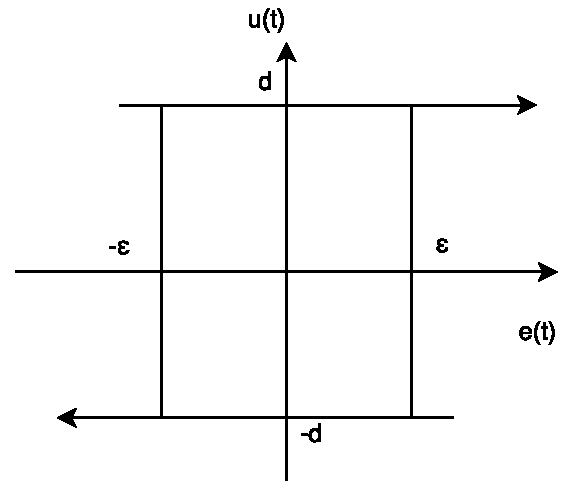
\includegraphics[width=0.4\linewidth]{rele_com_hist.pdf}}
	\end{center}
	\centering
	\small Fonte: autor (2017)
\end{figure}


	O relé sem histerese, Figura \ref{fig:reles}(a), pode ser modelado no domínio do tempo por:
	
\begin{verbatim}
	Se e(t) > 0 então u(t) = +d;
	Se e(t) < 0 então u(t) = -d;
\end{verbatim}

Já o relé com histerese de Figura \ref{fig:reles}(b) pode ser modelado no domínio do tempo por simples regras linguísticas descrevendo o comportamento da histerese conforme mostra a seguir, onde $\varepsilon$ é igual a \verb+eps+.

\begin{verbatim}
	Se |e(t)| > eps e e(t) > 0 então u(t) = +d;
	Se |e(t)| > eps e e(t) < 0 então u(t) = -d;
	Se |e(t)| < eps e u(t-1) = +d então u(t) = +d;
	Se |e(t)| < eps e u(t-1) = -d então u(t) = -d;
\end{verbatim}

	Considerando o relé sem histerese e com histerese, conforme mostra a Figura \ref{fig:reles}, têm-se as equações (\ref{eq:N(a)}) relatando as funções descritivas.
	
\begin{equation}
	\label{eq:N(a)}
	\begin{split}
	-1/N(a) 	&=	-{\pi}a/{4d} & (sem~histerese)\\
	-1/N(a) 	&=	-\pi\sqrt{a^2 {-\varepsilon}^2}/{4d} - j\pi\varepsilon/{4d} & (com~histerese)
	\end{split}
\end{equation}	

	A partir da modelagem do relé por função descritiva e da operação do sistema sob o controle do relé, pode-se determinar a função de transferência do processo por (\ref{eq:G(jw)}), onde $a$ é a amplitude de oscilação do sinal na saída do processo e $\omega$ é a frequência de oscilação medida.
	
\begin{equation}
	\label{eq:G(jw)}
	\begin{split}
	G_p(j\omega) 	&=	-{1/{N(a)}} &\\
	G_p(j\omega) 	&=	-{\pi}a/{4d} & (sem~histerese)\\
	G_p(j\omega) 	&=	-\pi\sqrt{a^2 {-\varepsilon}^2}/{4d} - j\pi\varepsilon/{4d} & (com~histerese)\\
	\end{split}
\end{equation}	

	Pela Equação (\ref{eq:G(jw)}), pode-se estimar a função de transferência do processo na frequência de cruzamento utilizando-se o relé sem histerese. A equação (\ref{eq:G(jw)}) permite também estimar a função de transferência do processo em diferentes frequências utilizando-se um relé com histerese e ajustando-se diferentes valores para o parâmetro $\varepsilon$. 
	
	
	As regras de sintonia propostas por \.{A}str\"{o}m consistem no seguinte:
\begin{enumerate}[leftmargin=2cm,label=\alph*)]
	\item sob o controle a relé, espera-se o sistema realimentado entrar em oscilação;
	\item utilizando a expressão da função descritiva do relé, estima-se o ganho crítico e o período da oscilação que o sistema teria sob controle proporcional. \.{A}str\"{o}m considerou, que nestas condições, o ganho N(A) de Equação (\ref{eq:N(a)}) do relé representa um valor bem aproximado do ganho crítico $K_{cr}$. Por este motivo $K_{cr}$ é feito igual a N(A);
	\item encontrada a sintonia através da Tabela \ref{tab:zieglenichols}, o sistema passa a controle PID, conforme mostra a Figura \ref{fig:controle_rele_pid}.
\end{enumerate}


\begin{table}[!htb]
	\centering
	\caption{\label{tab:zieglenichols}Regras de ajustes estabelecidos por Ziegler-Nichols}
		\begin{tabular}{c|ccc}
		\textbf{Tipo de Controlador} & \textbf{$K_p$} & \textbf{$T_i$} & \textbf{$T_d$} \\ 
		\hline 
		\textbf{P} & 0,5$K_{cr}$ & Infinito & Zero \\ 
		\hline 
		\textbf{PI} & 0,45$K_{cr}$ & 0,83$T_{cr}$ & Zero \\ 
		\hline 
		\textbf{PID} & 0,6$K_{cr}$ & 0,5$T_{cr}$ & 0,125$T_{cr}$ \\ 
		\end{tabular} 
\legend{Fonte: \citeonline{COELHO:2015}}
\end{table}
	

A técnica de realimentação do relé e utilizada para substituir o procedimento manual de tentativa e erro na sintonia de controladores PID. A Figura \ref{fig:controle_rele_pid} ilustra o princípio de implementação da técnica adaptativa \emph{auto-tunning}. Quando a malha de controle está em oscilação com o relé, os parâmetros PID são calculados e armazenados automaticamente e o sistema troca o bloco do relé para o do PID. 

\begin{figure}[!htb]
	\caption{\label{fig:controle_rele_pid}Diagrama de blocos do sistema para autossintonia dos parâmetros do Controlador PID - SISO}
	\begin{center}
		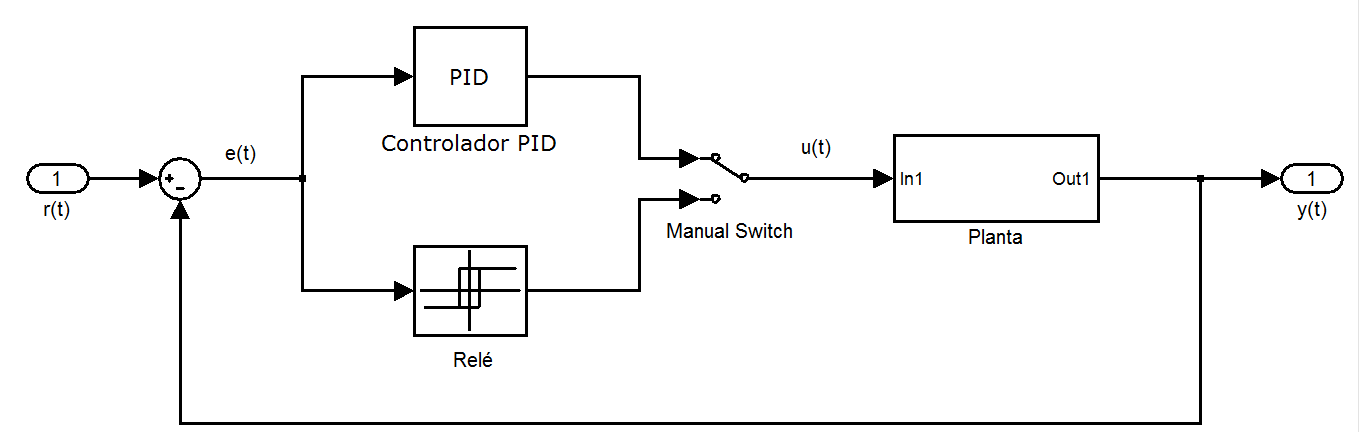
\includegraphics[width=.7\linewidth]{rele_pid.png}
	\end{center}
	\legend{Fonte: adaptado de \citeonline{barccante2011controle}}
\end{figure}
	\subsubsection{Método do Relé para sintonia do sistema SISO}
	Para exemplificar o método do relé, para o sistema motor-\textit{encoder} (SISO), foi determinado o ponto de cruzamento de ganho ou ponto crítico utilizando um relé (com e sem histerese) para a malha das rodas do Micromouse, e também traçado o diagrama de Nyquist para a malha de velocidade do robô para pelo menos 3 pontos distintos.

	O procedimento do método do relé para análise do processo SISO motor-\textit{encoder} foi feito a fim de verificar a curva de \emph{Nyquist}. No robô foi implementado um programa com o relé no domínio do tempo. A Figura \ref{fig:rele_siso} mostra o gráfico de entrada do processo e o gráfico em resposta ao relé para $\varepsilon$ de 1.

	Através da amplitude e período do sinal de saída $v$, para seus respectivos $\varepsilon$, foram encontrados os valores críticos, tanto de ganho como de período. Os valores de ganho crítico e período crítico para cada ponto do relé estão expostos na Tabela \ref{tab:k_u} e calculados conforme (\ref{eq:N(a)}), onde a margem de ganho $K_u$ é o inverso do módulo de $G(j\omega)$. 

\begin{figure}[!htb]
	\caption{\label{fig:rele_siso}Relé com histerese para $\varepsilon = 1$}
	\begin{center}
		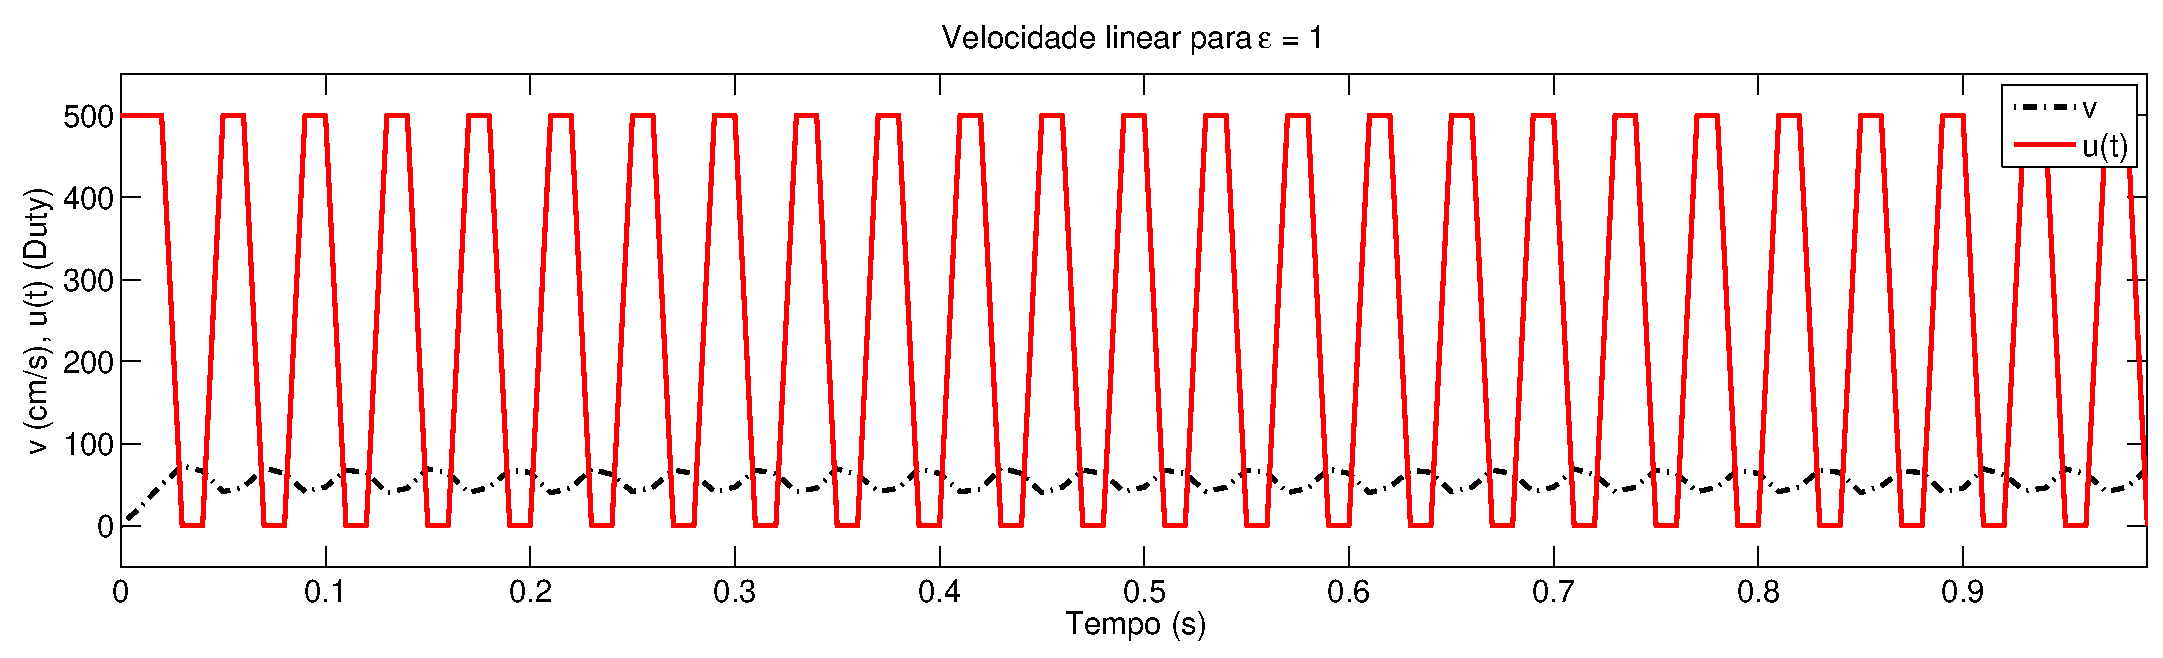
\includegraphics[width=.9\linewidth]{eps1.eps}
	\end{center}
	\legend{Fonte: autor (2017)}
\end{figure}

\begin{table}[!htb]
	\centering
	\caption{\label{tab:k_u}Margem de ganho $K_u$ e frequência crítica para relé com diversos $\varepsilon$. O valor de $d$ do relé é 250.}
		
	\begin{tabular}{c|ccccc}
	$\varepsilon$ & $a$ & $T_u (s)$ & $K_u$ & $\omega_u (rad/s)$ & $K_pK_u$\\ 
	\hline 
	\textbf{1} &  14.4893 & 0.04 & 22.0212 & 157.0796 & 4.8316 \\ 
	\hline 
	\textbf{20} & 30.3585 & 0.07 & 13.9369 & 89.7598 & 3.2758\\ 
	\hline
	\textbf{30} & 37.2581 & 0.09 & 14.4067 & 69.8132 & 3.1411\\ 
	\hline 
	\textbf{40} & 42.7779 & 0.11 & 20.9912 & 57.1199 & 4.5825\\ 
	\end{tabular} 
	
\legend{Fonte: autor (2017)}
\end{table}
	
\begin{figure}[!htb]
	\caption{\label{fig:nyquist_siso}Curva de \emph{Nyquist} para o sistema SISO do Micromouse}
	\begin{center}
		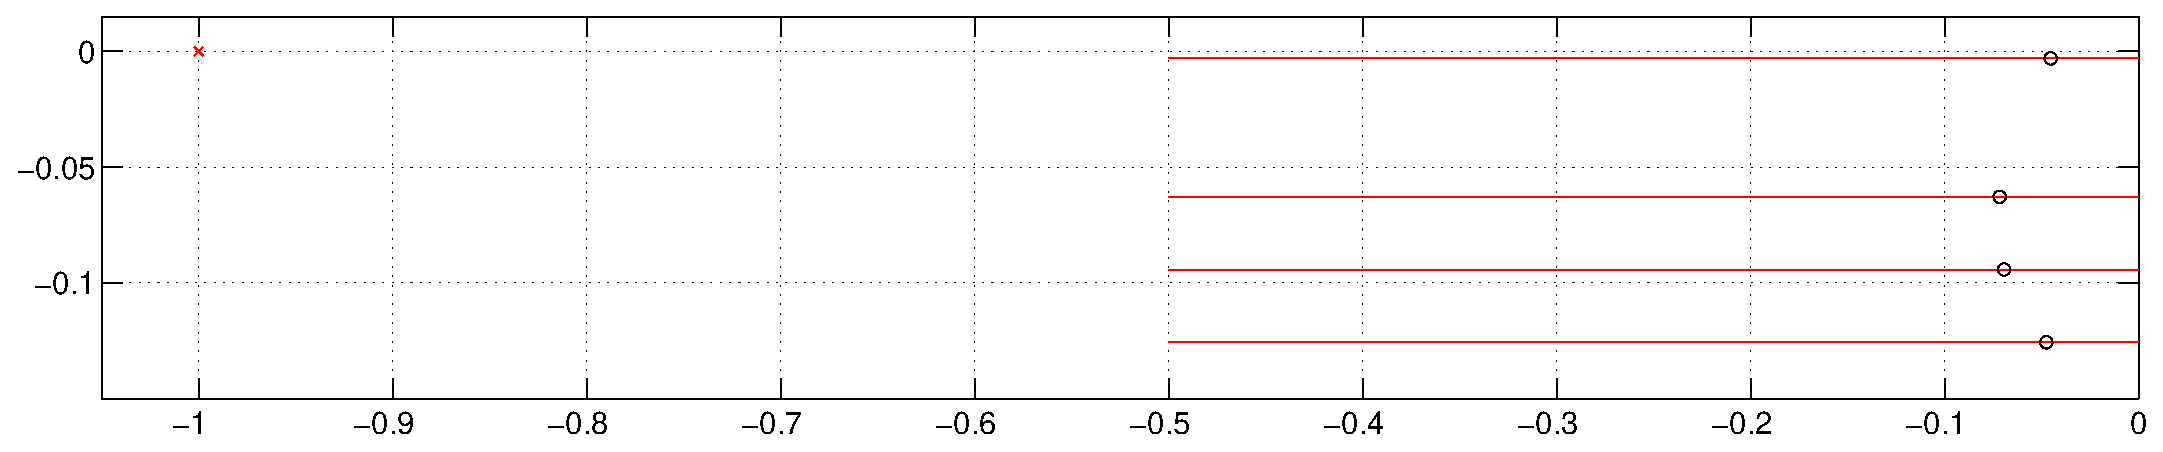
\includegraphics[width=.9\linewidth]{nyquist_pontos.eps}
	\end{center}
	\legend{Fonte: autor (2017)}
\end{figure}

	Pode-se observar que o processo é muito estável porque sua curva de Nyquist passa longe do ponto de instabilidade, como mostra a Figura \ref{fig:nyquist_siso}. Sua margem de ganho $K_u$ é de 22. As marcações em círculo são os pontos real e imaginário da Equação (\ref{eq:G(jw)}). As retas paralelas em vermelho representam a histerese para $\varepsilon$ de 1, 20, 30 e 40, respectivamente. Quanto maior a histerese, a reta paralela mais se desloca para baixo.

Por fim, calculou-se os parâmetros PID $k_P$, $k_I$ e $k_D$, da Equação (\ref{eq:pid}), utilizando a Tabela \ref{tab:zieglenichols} para os valores obtidos para relé com histerese de $\varepsilon = 1$ da Tabela \ref{tab:k_u}, que resultou na Tabela \ref{tab:zieglenichols_vel}. 
	
\begin{table}[!htb]
	\centering
	\caption{\label{tab:zieglenichols_vel}Parâmetros PID para a malha de velocidade baseados pela tabela do Ziegler-Nichols}
		\begin{tabular}{c|ccc}
		\textbf{Tipo de Controlador} & \textbf{$k_P$} & \textbf{$k_I$} & \textbf{$k_D$} \\ 
		\hline 
		\textbf{PID} & 13.2127 & 660.6347 & 0.0661 \\ 
		\end{tabular} 
\legend{Fonte: autor (2017)}
\end{table}


Estes valores foram utilizados no controlador discreto do Micromouse, e a robustez pode ser observada na Figura \ref{fig:PID_siso}. A saíde de velocidade segue a referência corretamente, com \textit{overshoots} esperados para entradas em degrau (mudança brusca de referência), e erro em regime permanente nulo com a inserção de um integrador através do PID. Os sinais de controle também estão enfatizados.

\begin{figure}[!htb]
	\caption{\label{fig:PID_siso}Saída de velocidade utilizando o os parâmetros PID do método Ziegler-Nichols}
	\begin{center}
		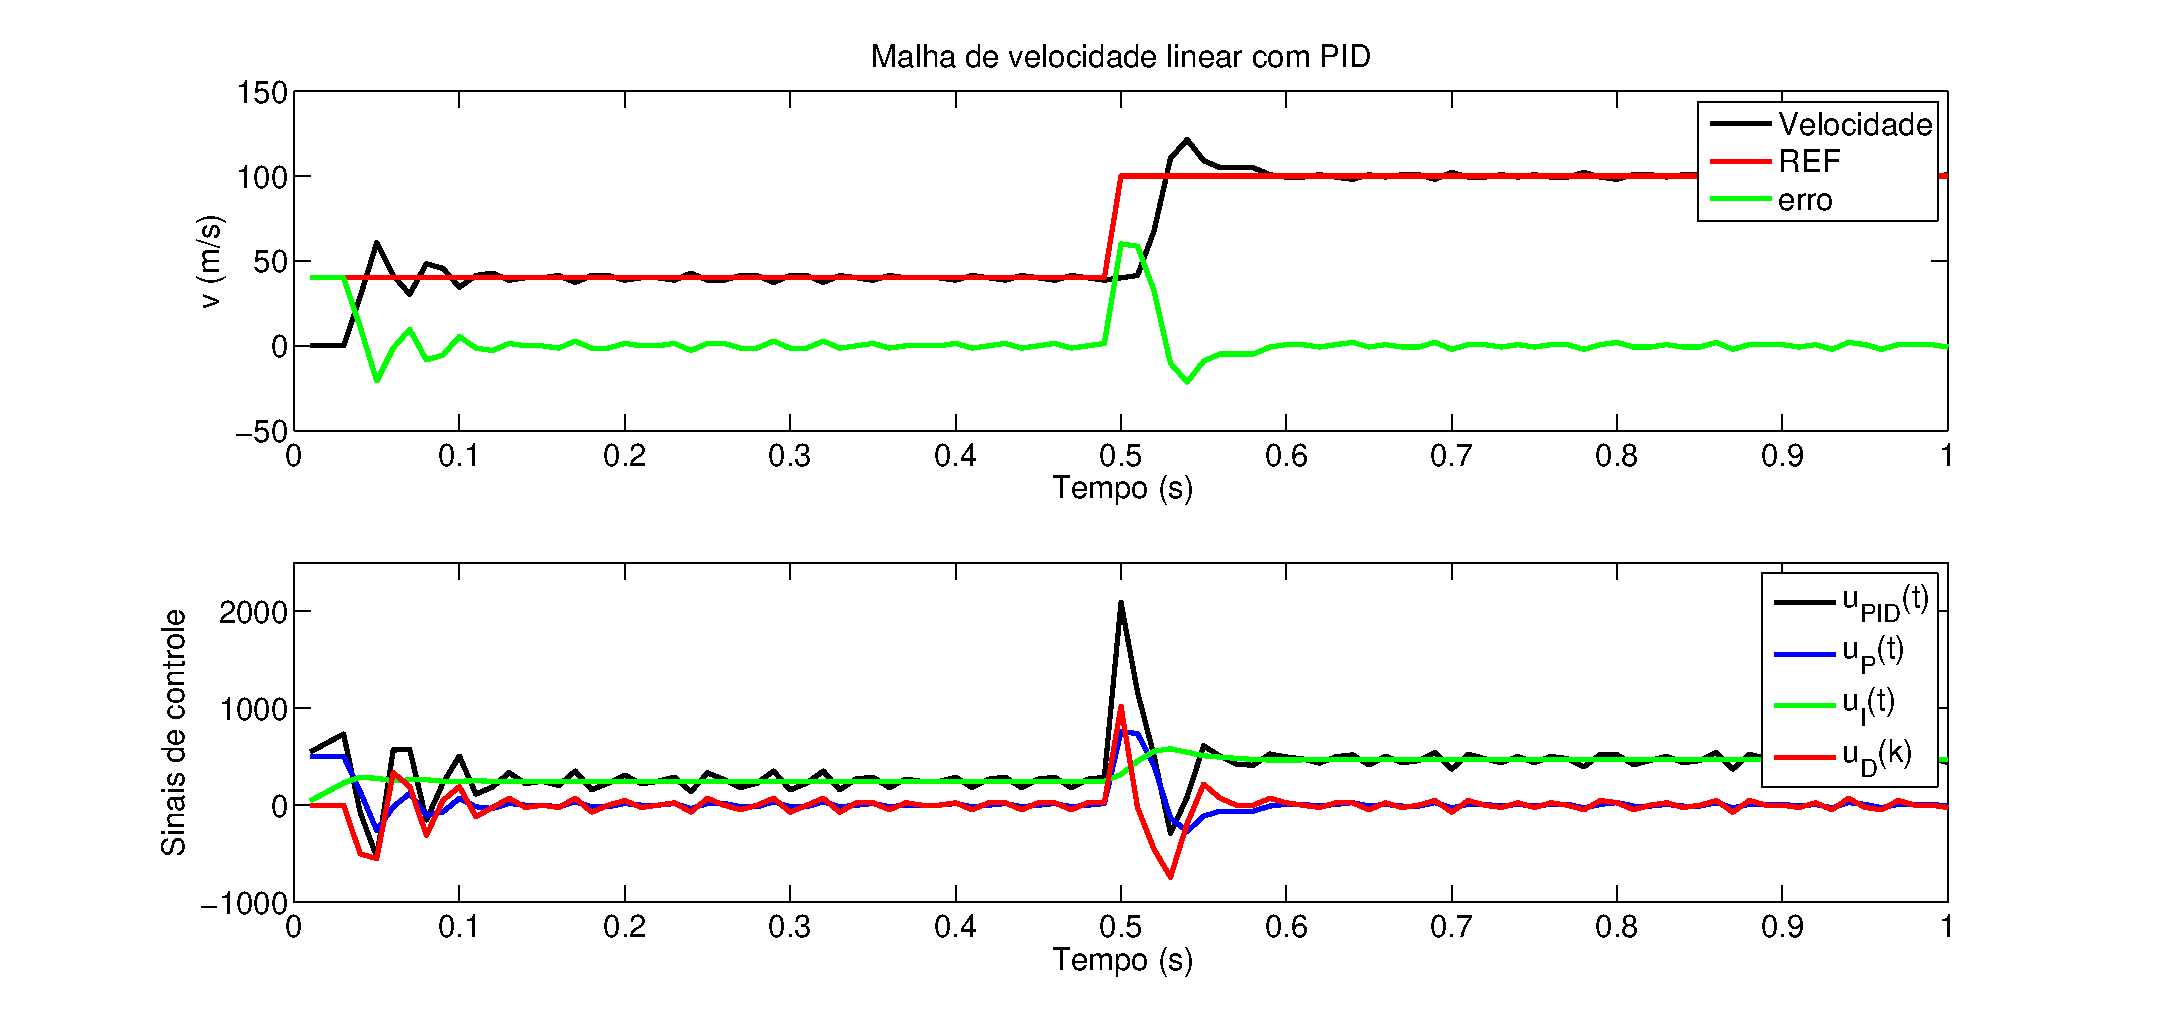
\includegraphics[width=.9\linewidth]{pid_vel.eps}
	\end{center}
	\legend{Fonte: autor (2017)}
\end{figure}

	\subsubsection{Método do Relé Sequencial para sintonia de sistemas MIMO}
	Segundo \citeonline{Tamura:2006}, muitas vezes, é difícil aplicar o método de autossintonia ao sistema MIMO (múltiplas entradas e múltiplas saídas), como é o do Micromouse, porque não é tão bem pesquisado como os sistemas SISO. Embora existam várias pesquisas do controle PID para o sistema MIMO, elas são restritas ao sistema de fase estável e/ou mínima em muitos casos.
	Os sistemas multivariáveis MIMO podem ser representados por matriz de funções de transferência \cite{katsuhiko2011engenharia}. Nesta representação, um sistema multivariável com $j$ entradas $u_1, u_2, ..., u_j$ e $i$ saídas $y_1, y_2,..., y_i$, que definem os vetores $Y$ de saídas e $U$ de entradas, são dadas por (\ref{eq:Y_U}).
	
\begin{equation}
\label{eq:Y_U}
Y = \left[ \begin{array}{c} y_1 \\ y_2 \\ \vdots \\ y_i \end{array} \right];
U = \left[ \begin{array}{c} u_1 \\ u_2 \\ \vdots \\ u_j \end{array} \right]
\end{equation}


Na forma matricial, considerando um sistema linear, controlável e observável, a matriz de transferência é dado por (\ref{eq:Y(s)_U(s)}).

\begin{equation}
\label{eq:Y(s)_U(s)}
\left[ \begin{array}{c} Y_1(s) \\ Y_2(s) \\ \vdots \\ Y_i(s) \end{array} \right] = \begin{bmatrix}
G_{11} & G_{12} & \cdots & G_{1j} \\ 
G_{21} & G_{22} & \cdots & G_{2j} \\ 
\vdots & \vdots & \ddots & \vdots \\ 
G_{i1} & G_{i2} & \cdots & G_{ij}
\end{bmatrix} \times
\left[ \begin{array}{c} U_1 \\ U_2 \\ \vdots \\ U_j \end{array} \right]
\end{equation}


A Equação (\ref{eq:Y(s)_U(s)}) fornece como resultado uma matriz de transferência de ordem $ixj$ e cada elemento individual $G_{ij}(s)$ de $G(s)$ representa a função de transferência da malha respectiva de controle $y_i - u_j$, que, por sua vez, relaciona a variável manipulada $u_j$ à variável controlada $y_i$. A Figura \ref{fig:mimo_2x2} apresenta o diagrama de blocos para esta representação de um sistema 2x2. $G_{21}(s)$ e $G_{12}(s)$ representam as interações entre as malhas do sistema.

\begin{figure}[!h]
	\caption{\label{fig:mimo_2x2}Diagrama de blocos do sistema MIMO $2x2$}
	\begin{center}
		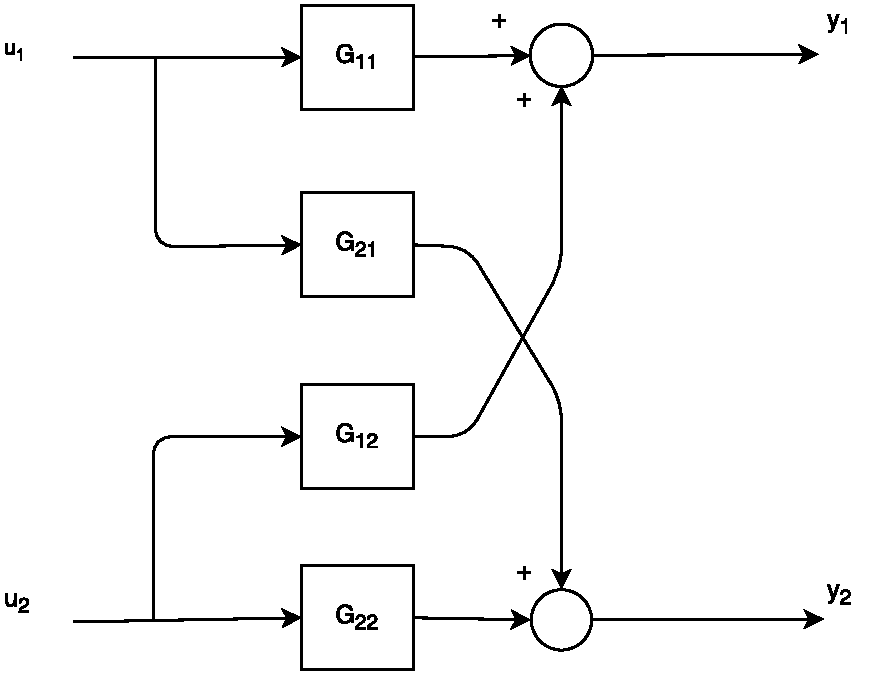
\includegraphics[width=.4\linewidth]{MIMO2x2.pdf}
	\end{center}
	\legend{Fonte: adaptado de \citeonline{barccante2011controle}}
\end{figure}

	
	
	\subsubsection{Identificação dos motores via Mínimos Quadrados Não-Recursivos}
	Considerando que o sistema motor-\textit{encoder} do robô seja caracterizado por uma entrada, $u(t)$, uma saída, $y(t)$, uma perturbação, $e(t)$, e com função de transferência discreta linear na forma (\ref{eq:eq_ordem}), cuja representação por uma equação a diferença pode ser vista em (\ref{eq:eq_dif_ordem}).
	

\begin{equation}
	\label{eq:eq_ordem}
	\begin{split}
	A(z^{-1})y(t) &= z^{-d}B(z^{-1})u(t)+e(t), onde \\
	A(z^{-1}) &= 1 + a_{1}z^{-1} + ... + a_{na}z^{-na}\\
	B(z^{-1}) &= b_0 + b_1z^{-1} + ... + b_{nb}z^{-nb}
	\end{split}
\end{equation}

\begin{equation}
	\label{eq:eq_dif_ordem}
	\begin{split}
	y(t) &= -a_1y(t-1) - a_2y(t-2) - ... - a_{na}y(t-na) + b_0u(t-d) + b_1u(t-d-1) + \\ &... + b_{nb}u(t-d-nb) + e(t)
	\end{split}
\end{equation}

Definindo o \emph{vetor de medidas}, $\phi(t)$, de dimensão $(na + nb + 1) \times 1$, Equação (\ref{eq:vet_med}), e o \emph{vetor de parâmetros}, $\theta(t)$, Equação (\ref{eq:vet_param}), de dimensão $(na + nb + 1) \times 1$, pode-se reescrever a Equação (\ref{eq:eq_dif_ordem}) como mostra a Equação (\ref{eq:eq_matr_ordem}), que é denominado \emph{modelo de regressão linear} \cite{COELHO:2015}.

\begin{equation}
	\label{eq:vet_med}
	\begin{split}
	{\varphi}^T(t) &= [-y(t-1)-y(t-2)...-y(t-na) u(t-d) ... u(t-d-nb)]
	\end{split}
\end{equation}

\begin{equation}
	\label{eq:vet_param}
	\begin{split}
	{\theta}^T(t) &= [a_1 \, a_2 \, ... \, a_{na} \, b_0 \, b_1 \, ... \, b_{nb}]
	\end{split}
\end{equation}

\begin{equation}
	\label{eq:eq_matr_ordem}
	\begin{split}
	y(t) &= \varphi^{T}(t)\theta(t) + e(t)
	\end{split}
\end{equation}

	Supondo que são realizadas $N$ medidas, suficientes para determinar os parâmetros $a_i$ e $b_i$, então tem-se as matrizes (\ref{eq:n_medidas}).
	
	
	\begin{equation}
\label{eq:n_medidas}
	\begin{split}
 \left[ \begin{array}{c} y(0) \\ y(1) \\ \vdots \\ y(N-1) \end{array} \right]  = \left[ \begin{array}{c} \phi^{T}(0) \\ \phi^{T}(1) \\ \vdots \\ \phi^{T}(N-1) \end{array} \right] \times \theta(t) + \left[ \begin{array}{c} e(0) \\ e(1) \\ \vdots \\ e(N-1) \end{array} \right]
	\end{split}
\end{equation}

\begin{equation}
\label{eq:eq_2_ordem}
	\begin{split}
G(z^{-1}) = \frac{z^{-1}(b_1 + z^{-1}b_2)}{1 + z^{-1}a_1 + z^{-2}a_2}
	\end{split}
\end{equation}

	A maioria dos processos reais pode ser modelado para ordem 2. Considerando (\ref{eq:eq_ordem}) com $na = nb = 2 $ e $d = 1$, o modelo de equação discreto \texttt{G(z)} de segunda ordem para os motores pode ser representado por (\ref{eq:eq_2_ordem}). A representação matricial de (\ref{eq:n_medidas}) está na Equação (\ref{eq:n_medidas2}), onde a matriz observação está em (\ref{eq:matriz_observ}), para sistema de segunda ordem, e o vetor de saída é dado por (\ref{eq:vetor_saida}), onde a matriz $\phi$ não é quadrada, isto é, tem mais linhas do que colunas.
	
	\begin{equation}
\label{eq:n_medidas2}
	\begin{split}
Y = \phi^{T}(t)\theta(t) + E
	\end{split}
\end{equation}

	\begin{equation}
\label{eq:vetor_saida}
	\begin{split}
Y^T = \left[y(0) y(1) y(2) \cdots y(N-1) \right]
	\end{split}
\end{equation}

\begin{equation}
\label{eq:matriz_observ}
	\begin{split}
		\phi = \left[\begin{matrix}
		-y(-1) & -y(-2) & u(-d) & u(d-1) \\ 
		-y(0) & -y(-1) & u(1-d) & u(-d)  \\ 
		-y(1) & -y(0) & u(2-d) & u(-d) \\
		\cdots & \cdots & \cdots & \cdots \\ 
		-y(N-2) & -y(N-3) & u(N-d-1) & u(N-d-2)
		\end{matrix} \right]
	\end{split}
\end{equation}

%\begin{equation}
%\label{eq:matriz_observ}
%	\begin{split}
%		\phi = \left[\begin{matrix}
%		-y(-1) & -y(-2) & \cdots & -y(-na) & u(-d) & u(d-1) & \cdots & u(-d-nb) \\ 
%		-y(0) & -y(-1) & \cdots & -y(1-na) & u(1-d) & u(-d) & \cdots & u(1-d-nb) \\ 
%		-y(1) & -y(0) & \cdots & -y(2-na) & u(2-d) & u(1-d) & \cdots & u(2-d-nb) \\ 
%		\cdots & \cdots & \cdots & \cdots & \cdots & \cdots & \cdots & \cdots \\ 
%		-y(N-2) & -y(N-3) & \cdots & -y(N-na-1) & u(N-d-1) & u(N-d-2) & \cdots & u(N-d-nb-1)
%		\end{matrix} \right]
%	\end{split}
%\end{equation}


	A estimativa do vetor de parâmetros, $\hat{\theta}$, pode ser obtida pelo procedimento dos mínimos quadrados, que resulta na Equação (\ref{eq:est_param}). O estimador dos mínimos quadrados (\ref{eq:est_param}) é uma transformação linear sobre Y (função linear das medidas) e, assim, é denominado \emph{estimador linear} \cite{COELHO:2015}. 
	
	\begin{equation}
\label{eq:est_param}
\hat{\theta} = [\phi^T\phi]^{-1}\phi^TY
\end{equation}

Na aplicação do estimador dos mínimos quadrados, todas as medidas foram coletadas e posteriormente analisadas, técnica de identificação \emph{offline}.
Uma entrada aleatória é gerada através da função \texttt{rand()}, em C, e a cada período de amostragem, o microcontrolador configura um novo valor aleatório para a entrada do processo. Os valores de entrada e saída são enviados para o \textit{MATLAB} e acumulados em vetor. Após feita a coleta, a matriz observação (\ref{eq:matriz_observ}) é gerada. Ao aplicar (\ref{eq:est_param}), os coeficientes de (\ref{eq:eq_2_ordem}) foram obtidos para os motores. Seus valores estão na Tabela \ref{tab:parametros_teta}.

\begin{table}[!htb]
	\centering
	\caption{\label{tab:parametros_teta}Parâmetros da função de transferência estimados para os motores (N = 200)}
	\begin{tabular}{cc|cc}
	$G_L(z)$ & Motor Esquerdo & $G_R(z)$ & Motor Direito \\ 
	\hline 
	$a_1$ & -0,5915 & $a_1$ & -0,6096 \\ 
	\hline 
	$a_2$ & -0,0767 & $a_2$ & -0,0654 \\ 
	\hline 
	$b_1$ & 0,0149 & $b_1$ & 0,0149 \\ 
	\hline 
	$b_2$ & 0,0142 & $b_2$ & 0,0131 \\ 
	\end{tabular} 
	
	\legend{Fonte: autor (2017)}
\end{table}

	\subsubsection{Sistema realimentado proposto}
	O sistema de controle proposto para o Micromouse é mostrado na Figura \ref{fig:mimo_pid}. O processo contém dois sistemas MIMO, em cascata, e dois blocos PID (um para a malha de velocidade linear e outro para a malha de velocidade angular), sugeridos por \citeonline{6734188}.

	Com a identificação da função de transferência dos motores, foi possível a simulação de toda a malha de controle no Simulink. 
	
\begin{figure}[!htb]
	\caption{\label{fig:mimo_pid}Diagrama de blocos do sistema MIMO proposto para o Micromouse com dois blocos PID em malha fechada}
	\begin{center}
		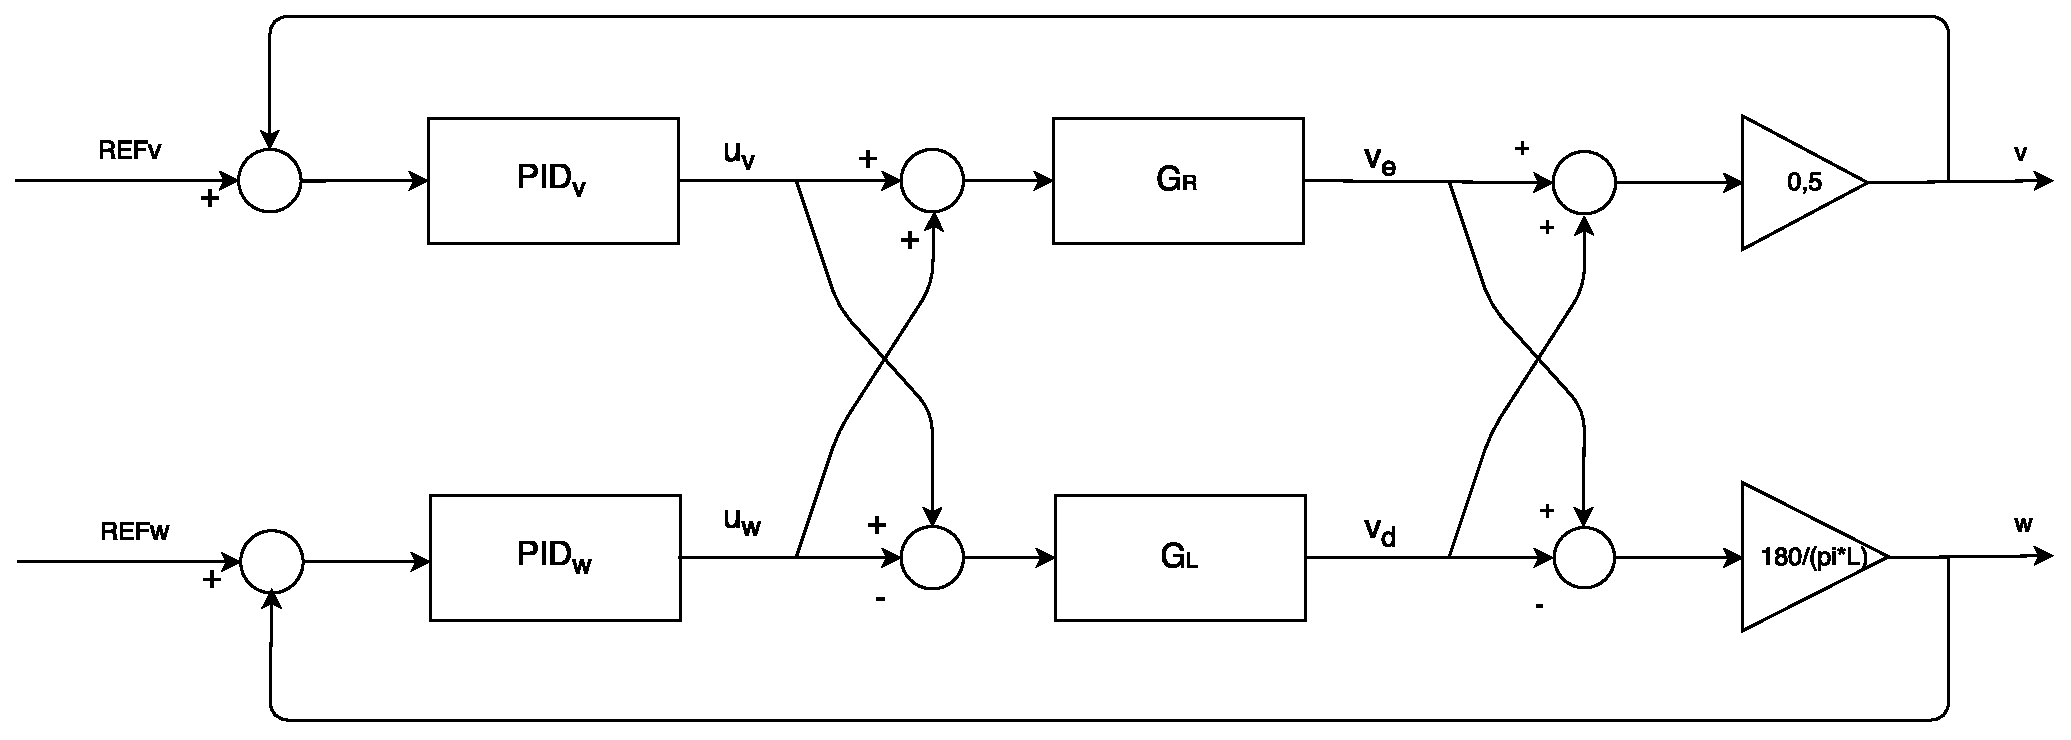
\includegraphics[width=1\linewidth]{MIMO_pid.pdf}
	\end{center}
	\legend{Fonte: autor (2017)}
\end{figure} 



Para identificação do processo e sintonia dos dois controladores, foram utilizados dois relés para sintonia em sequência, conforme sugere o trabalho de \citeonline{barccante2011controle}, para sistemas deste tipo.

A seguir, é apresentado o projeto dos perfis de curva e de velocidade, que são as entradas de referência do sistema do controle em \emph{malha fechada}. 

\subsection{Projeto de perfis de velocidade}
	O controlador proposto implementado é responsável por ajustar as saídas do processo através dos valores de referência do sistema MIMO. O robô poderá realizar qualquer tipo de trajetória, desde que se crie perfis de reta e de curva.
	
	Porém, os seguintes detalhes são importantes ao construir um perfil de curva:
	
	\begin{enumerate}[leftmargin=2cm,label=\alph*)]
	\item se a referência de velocidade linear é constante, e a referência de velocidade angular é nula, então o robô seguirá em frente com a mesma velocidade linear;
	\item em um sistema ideal, com aceleração infinita, se o robô deseja realizar uma curva com um raio $R$, e já com as velocidades de referência constante $v_0 \neq 0~m/s$ e $\omega_0 = 0 ~rad/s$, a velocidade angular de referência deverá sair de $\omega_0$ imediatamente para $\omega = (v_0/R)~rad/s$ no instante da curva;
	\item ao realizar certo ângulo $\theta$, a velocidade angular deverá sair imediatamente de $\omega$ para $\omega_0$, cessando o período de curva.
	\end{enumerate}
	
	Todavia, num sistema real, a velocidade angular não muda abruptamente, nem tampouco com controlador mais eficiente, como mostra a Figura \ref{fig:vel_rodas}(a). Uma solução alternativa e prática é acelerar uma roda e desacelerar a outra, de forma gradativa, como é mostrado na Figura \ref{fig:vel_rodas}(b).
	
\begin{figure}[!htb]
	\caption[Velocidades das rodas em uma curva]{\label{fig:vel_rodas}Velocidades das rodas em uma curva}
	\begin{center}
		\subfloat[Controle impossível]{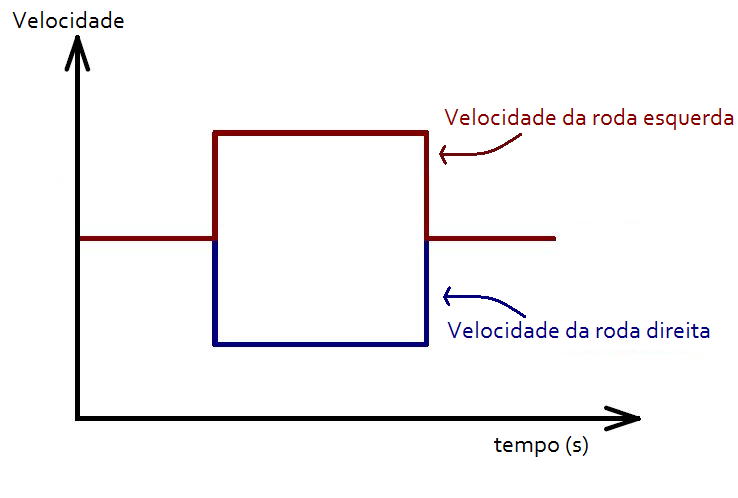
\includegraphics[width=0.4\linewidth]{curva_impossivel.png}}
		\hspace*{0.1\linewidth}
		\subfloat[Solução alternativa]{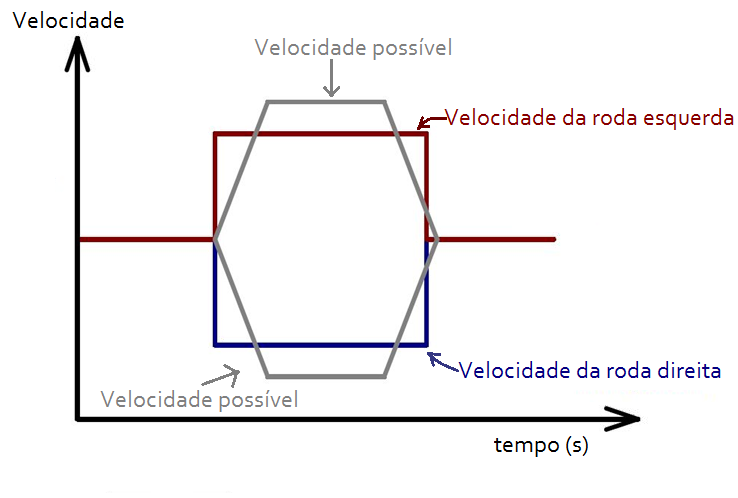
\includegraphics[width=0.4\linewidth]{curva_possivel.png}}
	\end{center}
	\centering
	\small Fonte: autor (2017)
\end{figure}
	
	\subsubsection{Curva desejada}
	
	O algoritmo utilizado é o \emph{Flood Fill tradicional}, que indica as direções \texttt{FRENTE}, \texttt{ESQUERDA}, \texttt{DIREITA} e \texttt{VOLTA}.  O sentido sempre é dado antes do robô entrar na próxima célula, como mostra a Figura \ref{fig:estados_robo}. Portanto, o robô só poderá realizar curvas de 90 graus, para curvas à esquerda e à direita, e um giro de 180 graus em seu próprio eixo quando o robô precisa retornar.

	Porém, como o robô precisa se posicionar de frente para a próxima célula para obter os obstáculos corretamente através dos sensores IR, após a curva, a trajetória semicircular, com o ponto de curvatura sobre o canto da célula, de raio igual à metade da largura da célula, conforme é mostrado na Figura \ref{fig:curvas_perfil}(a), deverá ser alterada para uma curva \emph{mais fechada}, conforme mostra a Figura \ref{fig:curvas_perfil}(b). Desta forma, o robô, ao terminar a curva, poderá ler os obstáculos ainda na célula anterior, com 3 cm de distância para a próxima célula.
	

\begin{figure}[!htb]
	\caption[Projeto de curvas]{\label{fig:curvas_perfil}projeto de curvas}
	\begin{center}
		\subfloat[Curva ideal]{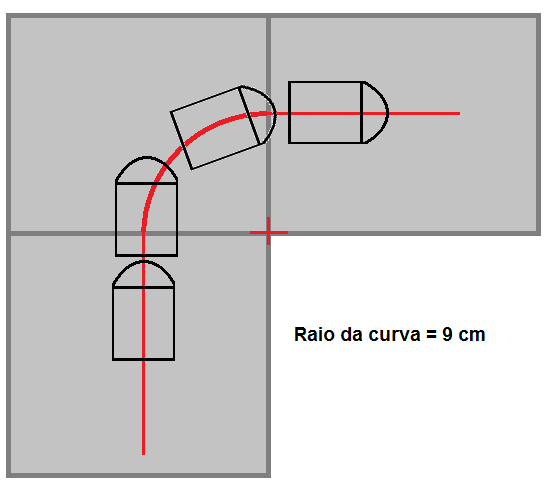
\includegraphics[width=0.4\linewidth]{curva_9cm.png}}
		\hspace*{0.1\linewidth}
		\subfloat[Curva proposta]{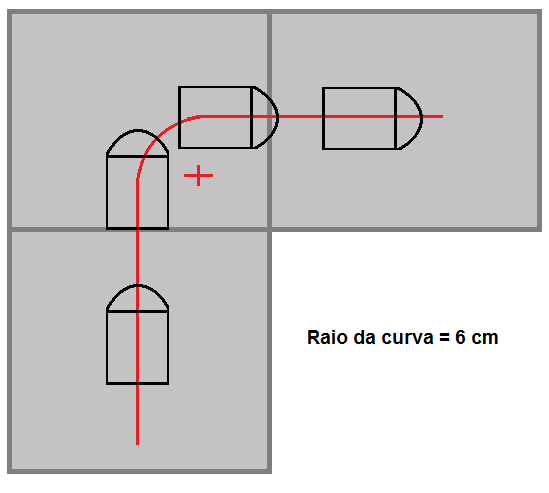
\includegraphics[width=0.4\linewidth]{curva_6cm.png}}
	\end{center}
	\centering
	\small Fonte: autor (2017)
\end{figure}


	\subsubsection{Determinando o perfil de curva de 90 graus}
	O robô sempre se moverá no labirinto com velocidade linear fixa, portanto, esta será a velocidade tangencial do movimento circular nos momentos de curva. Como o sistema não pode alterar abrubtamente a velocidade angular, a solução viável é a aceleração em rampa, conforme mostra o gráfico de velocidade a projetar da Figura \ref{fig:curvasperfil_1}. O ângulo $\theta$ feito pelo robô será o mesmo da trajetória ideal quando a área dos gráficos são iguais.

Diante dos fatos, os cálculos para determinar o tempo de curva e velocidade angular ideal são mostrados em (\ref{eq:traj_ideal}). O tempo de curva é baseado no gráfico de velocidade angular ideal e deve ser igual ao ângulo de curva desejado de 90 graus.

\begin{figure}[!htb]
	\caption{\label{fig:curvasperfil_1}Velocidade angular ideal x atual}
	\begin{center}
		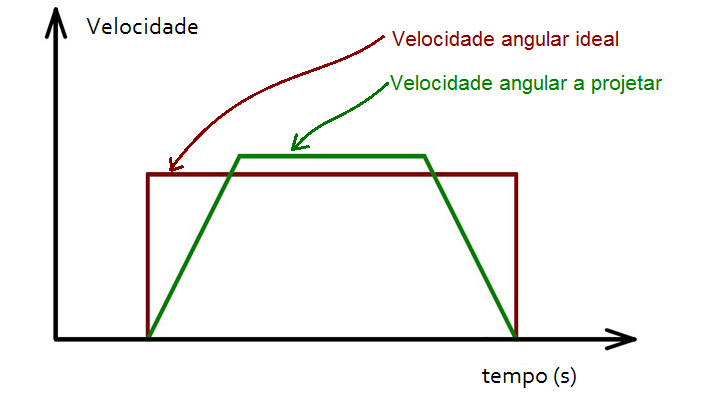
\includegraphics[width=0.7\linewidth]{vel_angular.png}
	\end{center}
	\legend{Fonte: autor (2017)}
\end{figure} 


\begin{equation}
\label{eq:traj_ideal}
	\begin{split}
	&\omega_{ideal} = (180 \times v_0)/(R \times \pi)\\
	&\theta_{curva} = 90^o\\
	&\theta_{curva} = \omega_{ideal} \times t_{curva} => t_{curva} = 90^o/\omega_{ideal}\\
	\end{split}
\end{equation}


\begin{figure}[!htb]
	\caption{\label{fig:curvasperfil_2}Visão geral do perfil de curva proposto}
	\begin{center}
		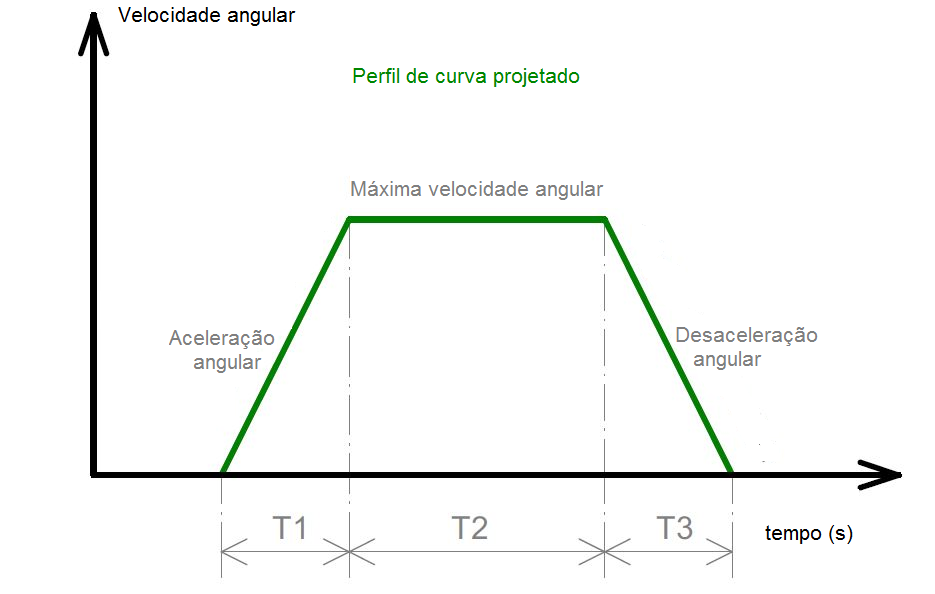
\includegraphics[width=0.7\linewidth]{perfildecurva.png}
	\end{center}
	\legend{Fonte: autor (2017)}
\end{figure} 

Com o tempo de curva, pode-se determinar a velocidade angular máxima do gráfico da Figura \ref{fig:curvasperfil_2}, considerando o tempo $T_1$ igual a $T_3$ e sendo 20\% do tempo de curva. Realizando a integral do gráfico de figura e igualando a 90 graus, tem-se $\omega_{max}$, conforme mostra (\ref{eq:traj_ideal2}).

\begin{equation}
\label{eq:traj_ideal2}
	\begin{split}
	&t_{curva} = T_1 + T_2 + T_3\\
	&T_1 = T_3 = 0.2 \times t_{curva}\\
	&T_2 = t_{curva} - 2 \times T_1 => T_2 = 0.6 \times t_{curva}\\
	&\omega_{max} = 90/(T_1 + T_2) ^o/s\\
	\end{split}
\end{equation}


	Portanto, para os tempos $T_1$ e $T_3$, a velocidade angular deverá ser incrementada e decrementada à taxa de $\omega_{max}T_s/T_1$, onde $T_s$ é a taxa de amostragem do sistema de controle, para o robô realizar uma curva de 90 graus. A diferença entre a curva à esquerda e a curva à direita é somente o sinal do $\omega_{max}$.
	
\subsubsection{Determinando o perfil de curva para giro de 180 graus em seu próprio eixo}

O giro em seu próprio eixo não precisa de um tempo fixo, como é necessário para a curva de 90 graus. A velocidade linear para giro é nula. Desta forma, as velocidades das rodas são forçadas a ter sinais trocados, conforme mostra a Figura \ref{fig:curvasperfil_3}. 

\begin{figure}[!htb]
	\caption{\label{fig:curvasperfil_3}O giro do robô em seu próprio eixo}
	\begin{center}
		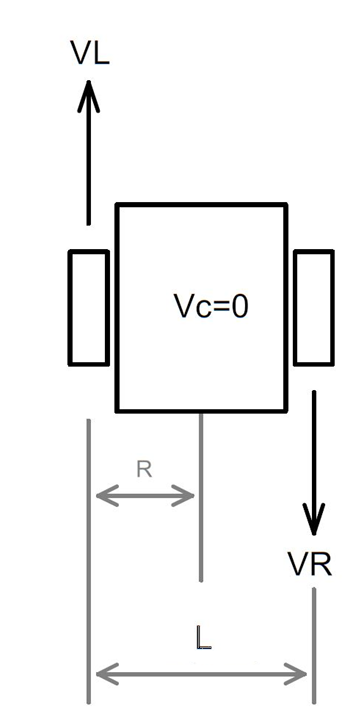
\includegraphics[width=0.2\linewidth]{giro180.png}
	\end{center}
	\legend{Fonte: autor (2017)}
\end{figure} 

Portanto, para o projeto Micromouse, o tempo para curva foi baseado no tempo $T_2$ do gráfico de Figura \ref{fig:curvasperfil_2}. Foi determinado que o robô deve girar 150 graus durante o tempo $T_2$ e 30 graus durante a aceleração e desaceleração da velocidade angular. As fórmulas para determinação dos tempos $T_1$, $T_2$ e $T_3$ para giro de 180 graus, bem como o tempo de curva, estão em (\ref{eq:traj_ideal_2}).

\begin{equation}
\label{eq:traj_ideal_2}
	\begin{split}
	&T_2 = 150/\omega_{max}\\
	&T_1 = T_3 = (15 \times 2)/\omega_{max}\\
	&t_{curva} = T_1 + T_2 + T_3\\
	\end{split}
\end{equation}

\subsubsection{Implementando os perfis no Micromouse}
Uma função chamada \verb+mover_robo()+ foi criada para executar os perfis de curva. Ela é sempre executada após o algoritmo de controle. Uma terceira máquina de estados foi criada, sendo que os estados são mudados após os tempos de rampa e de curva cessarem. Logo a seguir, são listados os estados e suas funções:
\begin{enumerate}[leftmargin=2cm,label=\alph*)]
\item \verb+RAMPA_VEL+: neste estado, o robô realizará uma aceleração constante de \textbf{velocidade linear}. Uma função \verb+rampa_vel()+ foi criada para realizar o incremento de velocidade de acordo com o tempo de rampa escolhido;
\item \verb+DESCIDA_VEL+: neste estado, o robô realizará uma rampa de desaceleração constante da velocidade linear. A mesma função para a rampa de aceleração é usada, porém, para decrementar o valor de velocidade por um tempo pré-determinado;
\item \verb+RAMPA_ANG+: o robô realizará uma rampa de \textbf{velocidade angular}. Uma função \verb+rampa_ang()+ foi criada para realizar o incremento de velocidade de acordo com o tempo de rampa escolhido;
\item \verb+DESCIDA_ANG+: neste estado, o robô realizará uma rampa de desaceleração constante da velocidade angular. A mesma função para a rampa de aceleração é usada, porém, para decrementar o valor de velocidade por um tempo pré-determinado;
\item \verb+MANTER_VEL+: este estado mantém o valor da velocidade linear por um tempo pré-determinado;
\item \verb+MANTER_ANG+: este estado mantém o valor da velocidade angular por um tempo pré-determinado.
\end{enumerate}

A Tabela \ref{tab:maquina_estado1} mostra a máquina de estado principal, controlado pelo algoritmo \emph{Flood Fill}, e como ocorre a transição dos estados da submáquina de estados para criação dos perfis de curva e de reta.

\begin{table}[!htb]
	\centering
	\caption{\label{tab:maquina_estado1}Máquinas de estado para geração dos perfis de reta e de curva}
\begin{tabular}{c|c|c|c}
 \multicolumn{2}{c|}{\textbf{Máquina de estado}} & \multicolumn{2}{c}{\textbf{Submáquina de estado}} \\ 
 \hline 
 \textbf{estados} & \textbf{estado inicial} & estado & próximo estado \\ 
 \hline 
 \verb+FRENTE+ & Se $v = 0$, \verb+RAMPA_VEL+  & \verb+RAMPA_VEL+ & \verb+MANTER_VEL+ \\ 
 \hline 
 • & Se $v\neq0$, \verb+MANTER_VEL+ & \verb+MANTER_VEL+ & \textbf{FLOODFILL} \\ 
 \hline 
 \verb+ESQUERDA+ & \verb+MANTER_VEL+ & \verb+RAMPA_ANG+ & \verb+MANTER_ANG+ \\ 
 \hline 
 • & • & \verb+DESCIDA_ANG+ & \textbf{FLOODFILL} \\ 
 \hline 
 • & • & \verb+MANTER_VEL+ & \verb+RAMPA_ANG+ \\ 
 \hline 
 • & • & \verb+MANTER_ANG+ & \verb+DESCIDA_ANG+ \\ 
 \hline 
 \verb+DIREITA+ & \verb+MANTER_VEL+ & \verb+RAMPA_ANG+ & \verb+MANTER_ANG+ \\ 
 \hline 
 • & • & \verb+DESCIDA_ANG+ & \textbf{FLOODFILL} \\ 
 \hline 
 • & • & \verb+MANTER_VEL+ & \verb+RAMPA_ANG+ \\ 
 \hline 
 • & • & \verb+MANTER_ANG+ & \verb+DESCIDA_ANG+ \\ 
 \hline 
 \verb+VOLTA+ & \verb+DESCIDA_VEL+ & \verb+RAMPA_VEL+ & \textbf{FLOOD FILL} \\ 
 \hline 
 • & • & \verb+RAMPA_ANG+ & \verb+MANTER_ANG+ \\ 
 \hline 
 • & • & \verb+DESCIDA_VEL+ & \verb+MANTER_VEL+ \\ 
 \hline 
 • & • & \verb+DESCIDA_ANG+ & \verb+RAMPA_VEL+ \\ 
 \hline 
 • & • & \verb+MANTER_VEL+ & \verb+RAMPA_ANG+ \\ 
 \end{tabular}  
	
	\legend{Fonte: autor (2017)}
\end{table}


Por exemplo, considerando uma velocidade linear $~v$ de $30 ~cm/s$, e raio de curva $~R$ de $6 ~cm$, e utilizando as fórmulas (\ref{eq:traj_ideal}) a (\ref{eq:traj_ideal_2}), tem-se o perfil de curva dos estados da máquina de estados da Tabela \ref{tab:maquina_estado1} ao longo do domínio do tempo, e a Figura \ref{fig:curvasperfil_4} mostra a visão geral do perfil de curva.

\begin{figure}[!htb]
	\caption{\label{fig:curvasperfil_4}Visão geral dos perfis de curva para os quatro estados}
	\begin{center}
		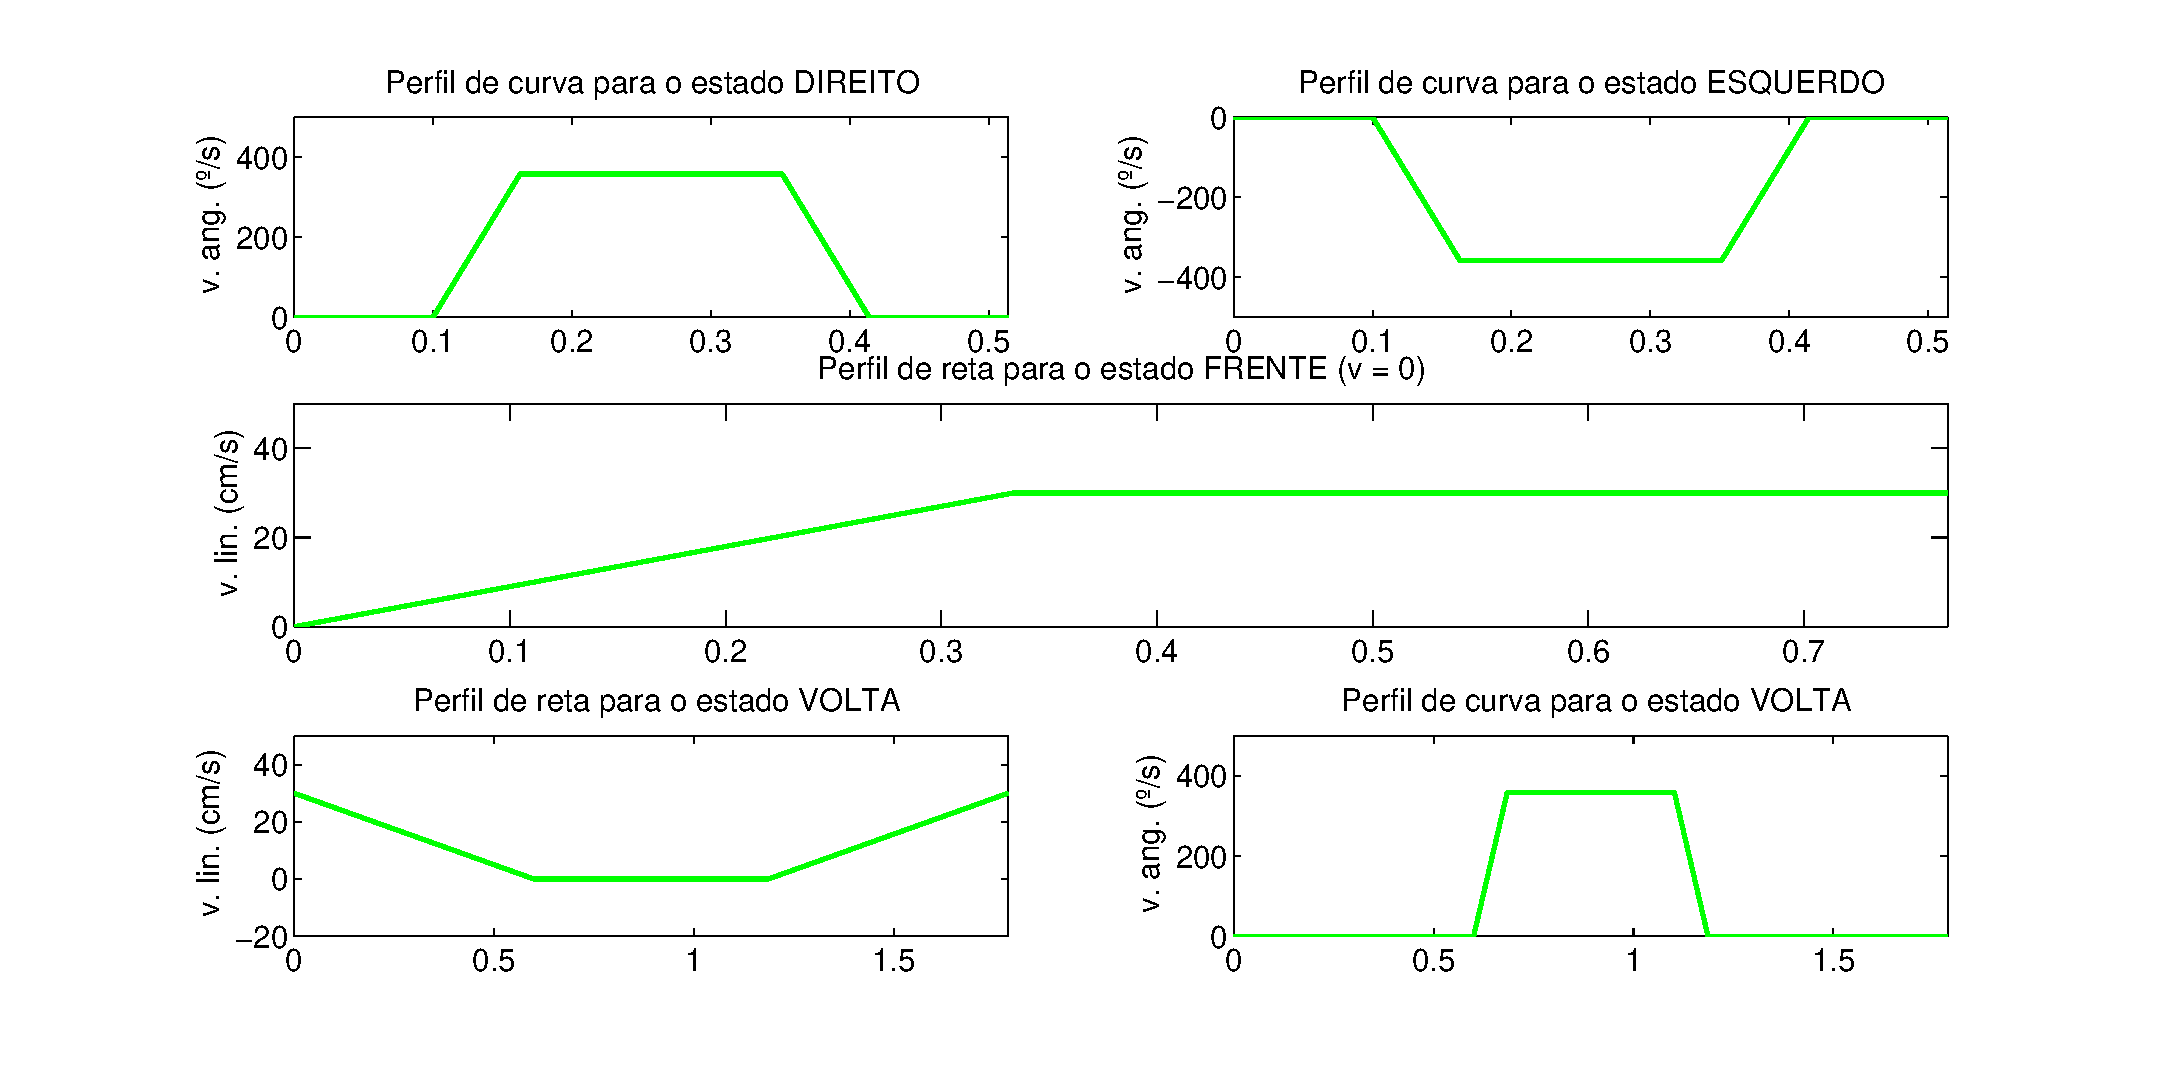
\includegraphics[width=1\linewidth]{perfisdecurva.eps}
	\end{center}
	\legend{Fonte: autor (2017)}
\end{figure} 

Então, cada estado da máquina de estados será responsável por modificar as entradas de referências do controle MIMO proposto, sendo que cada estado tem um tempo pré-determinado. 
\subsection{Controle dos erros de posicionamento no labirinto}
Numa trajetória real, os controladores estão expostos a ruídos iminentes do sistema. Com isto, em \emph{malha aberta}, o robô poderá sair da sua trajetória, acumulando erros de posicionamento ao longo do caminho. Derrapagens das rodas também causam erros deste tipo. A Figura \ref{fig:errosposic} mostra os dois erros de posicionamento do Micromouse, que devem ser corrigidos.

\begin{figure}[!htb]
	\caption{\label{fig:errosposic}Os erros de posicionamento do Micromouse no Labirinto}
	\begin{center}
		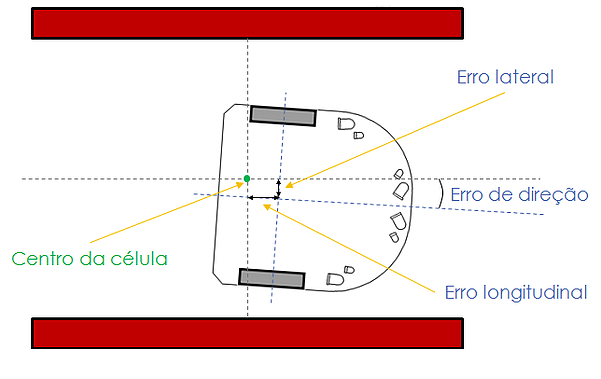
\includegraphics[width=0.6\linewidth]{sensor_feedback34png.png}
	\end{center}
	\legend{Fonte: adaptado de \citeonline{umart:2015}}
\end{figure} 

Os sensores IR poderão servir como \emph{feedback}. O robô, ao longo do percurso, sempre encontrará paredes. Com base nos valores das distâncias do robô às paredes, um sinal de controle entra como referência na entrada de velocidade angular, corrigindo, desta forma, a sua posição.

Os sensores tem os seguintes valores de tensão (em mV), quando o robô está centralizado:
\begin{enumerate}[leftmargin=2cm,label=\alph*)]
\item o sensor \textbf{l}, diagonal esquerdo, tem valor de tensão de 700 mV;
\item o sensor \textbf{r}, diagonal direito, tem valor de tensão de 1150 mV.
\end{enumerate}


Se o robô estiver mais à esquerda (Figura \ref{fig:feedback_IR}(a)), a velocidade angular deverá ser positiva para o robô desviar para o centro. Caso esteja mais à direita  (Figura \ref{fig:feedback_IR}(c)), o sinal de velocidade angular é negativo. O sinal de controle pelos sensores IR deverá ser nulo quando na posição correta (Figura \ref{fig:feedback_IR}(b)).


\begin{figure}[!htb]
	\caption[Sensores como feedback para correção da posição]{\label{fig:feedback_IR}Sensores como feedback para correção da posição no labirinto}
	\begin{center}
		\subfloat[Robô mais à esquerda]{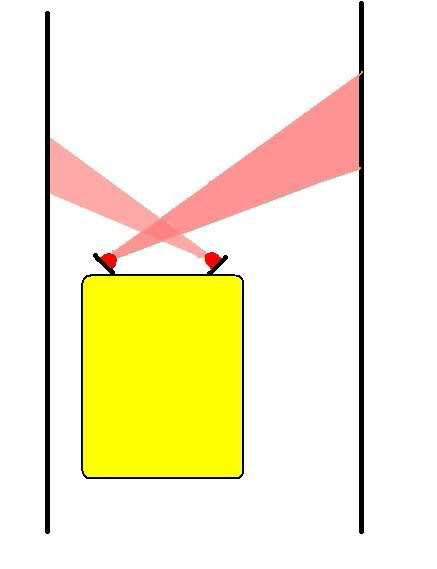
\includegraphics[width=0.2\linewidth]{sensor_feedback2.png}}
		\hspace*{0.1\linewidth}
		\subfloat[Robô centralizado]{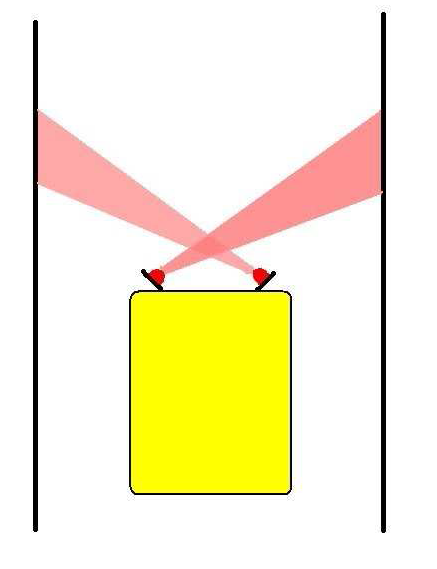
\includegraphics[width=0.2\linewidth]{sensor_feedback3.png}}
		\hspace*{0.1\linewidth}
		\subfloat[Robô mais à direita]{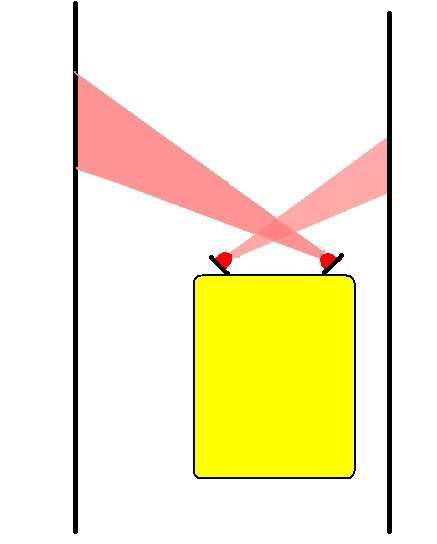
\includegraphics[width=0.2\linewidth]{sensor_feedback.png}}
	\end{center}
	\centering
	\small Fonte: adaptado de \citeonline{BORGES:2013}
\end{figure}


A partir desta informação, caso tenha paredes laterais no percurso, os sensores poderão alimentar a referência através de um controlador proporcional, como mostra a tabela \ref{tab:controlador_IR}.


\begin{table}[!htb]
	\centering
	\caption{\label{tab:controlador_IR}Controlador proporcional para o \emph{feedback} dos sensores IR}
\begin{tabular}{c|cc}
Condição & \multicolumn{2}{c}{Controle} \\ 
\hline 
\textbf{Parede à esquerda} & $u_{IR} = (l - 700) \times K_P;$ & $REF_w = u_{IR};$ \\ 
\hline 
\textbf{Parede à direita} & $u_{IR} = (1148 - r) \times K_P$; & $REF_w = u_{IR};$ \\ 
\end{tabular} 
	
	\legend{Fonte: autor (2017)}
\end{table}


\section{Observações finais}
Neste capítulo foram abordadas as características de projeto das partes principais que compõem um projeto Micromouse. O \autoref{Resultados} segue com os resultados observados nas simulações do algoritmo e controle implementados e, em seguida, da união deles com o robô. Discussões acerca desses resultados são feitas, bem como análises pertinentes a respeito dos algoritmos executados durante o percurso real em labirinto.


